\documentclass[pre,twocolumn,twoside,superscriptaddress,floatfix, aps, 10pt]{revtex4-1}

\usepackage{currfile}
\lefthyphenmin=3
\righthyphenmin=2

\usepackage{graphicx,epsfig,verbatim,enumerate}
\usepackage{amssymb,amsmath}
\usepackage{ifthen}

% Fonts and typesetting settings
\usepackage[sc]{mathpazo}
\usepackage[T1]{fontenc}
\linespread{1.05} % Palatino needs more space between lines
\usepackage{microtype}
\usepackage{textcomp}

\usepackage{longtable}

\usepackage{mathtools}

\newboolean{twocolswitch}

\newcommand{\www}[1]{\url{#1}}
\newcommand{\req}[1]{(\ref{#1})}
\newcommand{\Req}[1]{Eq.~(\ref{#1})}

% Lettrines
\usepackage{lettrine}

%useful shortcuts
\def\R{\ensuremath{\mathbb{R}}} %\ensuremath adds math mode, if forgotten
\def\Q{\ensuremath{\mathbb{Q}}}
\def\N{\ensuremath{\mathbb{N}}}
\def\Z{\ensuremath{\mathbb{Z}}}
\def\C{\ensuremath{\mathbb{C}}}

%shorcuts with arguments
\newcommand{\abs}[1]{\left\vert#1\right\vert} %nice absolute values
\newcommand{\bt}[1]{\textbf{#1}} %bold
\newcommand{\eq}[1]{\begin{align*}#1\end{align*}} %aligned equations
\newcommand{\norm}[1]{\left\lVert#1\right\rVert} %vector norm
\renewcommand{\eq}[1]{\begin{align*}#1\end{align*}} %aligned equations

%piecewise function

%\begin{displaymath}
%   f(x) = \left\{
%     \begin{array}{lr}
%       1 & : x \in \mathbb{Q}\\
%       0 & : x \notin \mathbb{Q}
%     \end{array}
%   \right.
%\end{displaymath} 


%environment
\newcommand{\tab}{\phantom{ssss}}

\usepackage{hyperref}
\usepackage{color}
\newcommand{\todo}[1]{\noindent\textcolor{blue}{{$\Box$ #1}}}

%colors
\definecolor{javagreen}{rgb}{0.25,0.5,0.35} %dark green color
\definecolor{lightblue}{rgb}{0.149,0.545,0.824} %solarized blue
\definecolor{sred}{rgb}{0.863, 0.196, 0.184} %solarized red

\newcommand{\blue}[1]{{\leavevmode\color{lightblue}{#1}}} %solarized blue 
\newcommand{\green}[1]{{\leavevmode\color{javagreen}{#1}}} %command for green
\newcommand{\red}[1]{{\leavevmode\color{sred}{#1}}} %solarized red
\newcommand{\gray}[1]{{\leavevmode\color[gray]{0.5}{#1}}} %gray text
\newcommand{\Prob}[1]{{\rm Pr}\left(#1\right)}


\setboolean{twocolswitch}{true}


\begin{document}

\title{\protect
Connecting Every Bit of Knowledge: \\
Wikipedia's First Link Network Unravelled
}

\author{
\firstname{Mark}
\surname{Ibrahim}
}
\email{mark.s.ibrahim@uvm.edu}

\affiliation{Department of Mathematics \& Statistics, 
    Computational Story Lab,  \\
    Vermont Complex Systems Center,
    Vermont Advanced Computing Core,
    The University of Vermont, Burlington, VT 05401.}

\author{
\firstname{Christopher}
\surname{M. Danforth}
}
\email{chris.danforth@uvm.edu}

\affiliation{Department of Mathematics \& Statistics, 
    Computational Story Lab,  \\
    Vermont Complex Systems Center,
    Vermont Advanced Computing Core,
    The University of Vermont, Burlington, VT 05401.}

\author{
\firstname{Peter}
\surname{Sheridan Dodds}
}

\email{peter.dodds@uvm.edu}

\affiliation{Department of Mathematics \& Statistics, 
    Computational Story Lab,  \\
    Vermont Complex Systems Center,
    Vermont Advanced Computing Core,
    The University of Vermont, Burlington, VT 05401.}

\begin{abstract}
  \protect
Apples, oranges, and the most obscure Dylan song too---is every topic a few clicks from Philosophy? 
Within Wikipedia, the surprising answer is yes: nearly all 
paths lead to Philosophy.
Wikipedia is the largest, most meticulously indexed collection of human knowledge ever amassed. 
More than information about a topic though, Wikipedia is a web of naturally emerging relationships.  
By following the First Link in an article, we connect entries to form a directed network: Wikipedia's First Link Network. 
Here we study the English edition of Wikipedia's First Link Network for insight into how the many topics, ideas, people, objects, and events
are related and organized.  


We algorithmically parse all 4.7 million articles to construct a map of Wikipedia's First Link Network. 
In a novel approach to uncover structure, we traverse every possible path through the network, 
measuring the accumulation of First Links, path lengths, basins, cycles, and even the influence a particular article exerts in shaping the 
network.
We discover many scale-free distributions, find Philosophy at a salient center, and uncover a flow from specific to general 
culminating around fundamental notions such as Community, State, and Science. 
Curiously, we also observe a gravitation towards topical articles including Health Care and Fossil Fuel.
These findings enrich our view of how we connect and structure
an ever growing load of information.
 
\end{abstract}

\maketitle



\section{Introduction}

Wikipedia is a towering achievement of the modern era. 
At no point in history has a larger or more meticulously indexed collection of human knowledge 
existed.
Wikipedia contains 37 million articles in 283 languages, 
with coverage spanning everything from little known ancient battles to the latest pharmaceutical drugs 
\cite{drugs} 
\cite{stats}.
All this information does not lie dormant. 
Wikipedia is the sixth most visited
site in the world, surpassing 18 billion page views and 26 million edits in a single month
\cite{wiki_edits}
\cite{wiki_views}.
The most widely used general reference, Wikipedia has amassed an awe-inspiring collection of human knowledge.

It's not surprising then to see Wikipedia as the object of many studies. 
Researchers have examined the cultural dynamics among editors
\cite{editors},
the accuracy of the content relative to traditional encyclopedias
\cite{accuracy1}
\cite{accuracy2},
the topics covered 
\cite{coverage},
and bias against portions of the population
\cite{bias_women}.
Wikipedia's content has also proven a powerful tool. 
Researchers have used Wikipedia to identify missing dictionary entries
\cite{missing_entries},
cluster short text
\cite{clustering},
compute semantic relatedness
\cite{semantic_relatedness},
and disambiguate meaning \cite{disambiguating}.

While these many studies have dissected and fruitfully applied Wikipedia's content,
few have examined the connections among the many articles.
Beyond information, Wikipedia is a web 
relating ideas. 
Within the body text of Wikipedia articles, hyperlinks reference
other Wikipedia articles.
A hyperlink from one Wikipedia article to another
indicates a relationship between the two articles
\cite{relevance}.
The notion that hyperlinks convey information about the content of a
page has proved successful in numerous domains from search engine algorithms 
such as PageRank 
\cite{pagerank} 
to topic classification
\cite{classifier}.
We treat a hyperlink as a mechanism connecting two ideas. 

The authors of a Wikipedia article choose where and whether to include a 
reference to another Wikipedia article
in the HTML markup.
In describing a particular topic, the authors decide which other articles are most
relevant references.
For example, the authors of the 
\href{https://en.wikipedia.org/wiki/Train}{"Train"}
article chose
"Rail Transport," "Cargo," and "Passengers" 
as pertinent articles to reference in describing trains
\cite{wiki_train}
.
The collection of hyperlinks emerges from the independent choice of each article's authors. 
The first hyperlink to another Wikipedia article marks the earliest moment in the body text where the authors
choose to connect the information discussed to that of another article.
By following the first hyperlink to another article in the English edition of
Wikipedia, we connect the ideas in one article to those in another, ultimately forming a directed network: 
{\it Wikipedia's First Link Network} (FLN).

\begin{figure*}[tp!]
  \centering	
  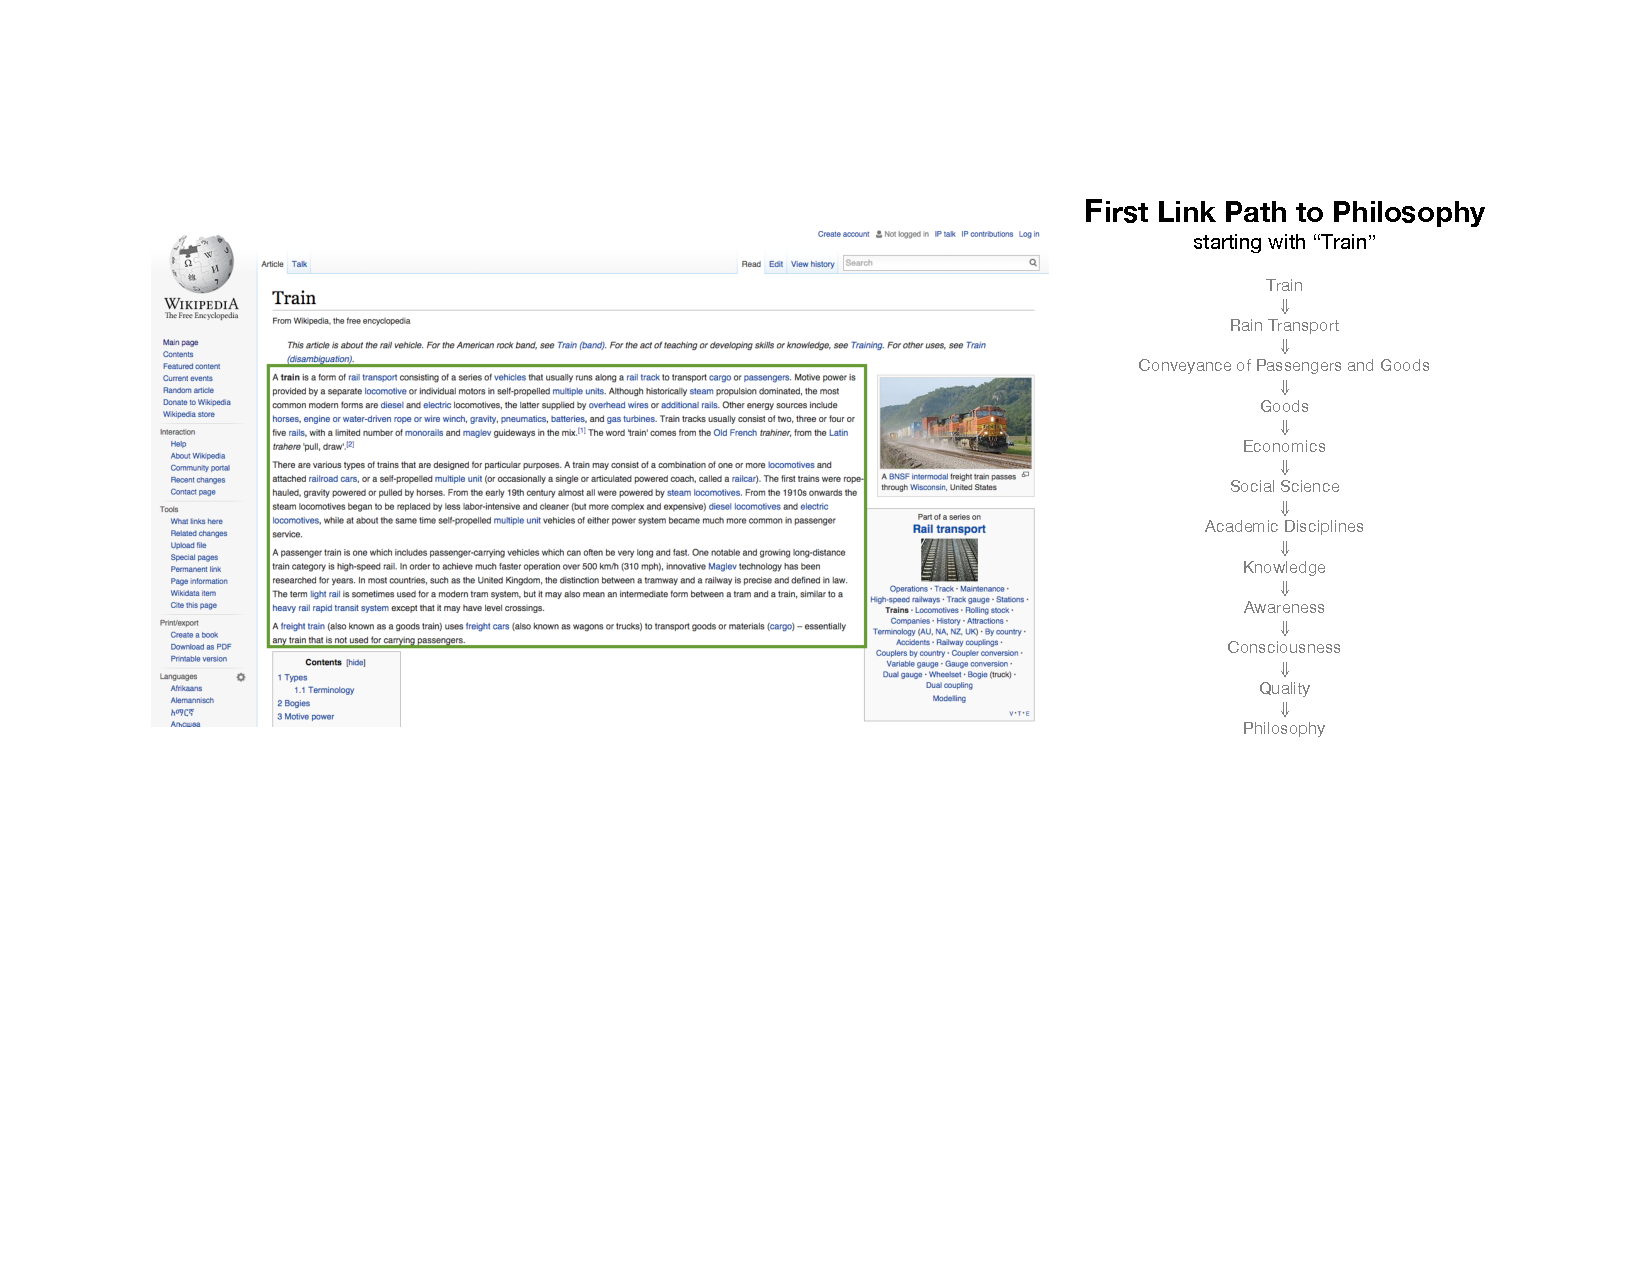
\includegraphics[width=\textwidth]{graphics/Train.pdf}  
  \caption{
    \textbf{First Link Path For "Train".}
    We follow the First Link to another Wikipedia article
    in the main body of the article---the area
    inside the green rectangle, which excludes 
    side bar elements, the navigation bar and title. 
    In this example, the First Link to another Wikipedia article is "Rail Transport." 
    We can again select the First Link on the "Rail Transport"
    article, repeating the process to 
    form a path of First Links.
  }
  \label{fig:Train First Links}
\end{figure*}

What information could the First Links possibly reveal?
Inspired by the claim that the majority of First Links lead to the 
"Philosophy" article---popularized by an 
\href{https://xkcd.com/903/}{xkcd}
comic and subsequently
discussed in blog posts 
\cite{mat_blog, Ilmari_first_links, xkcd}
---we holistically study 
Wikipedia's FLN as a map relating areas of human knowledge. 
The map is a hierarchical taxonomy where, for example, "Train" links to a parent node, 
"Rail Transport," while many child nodes, "Steel" and "Horsepower," link to 
"Train." Unlike previous taxonomies
created by individuals
\cite{locke, descartes, aristotle}
or a select group of individuals 
\cite{hist_thesaurus}, 
the organization of ideas in the FLN 
does not emerge from a concerted or a centralized effort. 
Rather each link in the FLN emerges from the choice of each author.
Collectively, the FLN is a wealth of relations among inventions, places,
figures, objects, and events across space and time.


Our goal is to study the structure of the FLN for insight into how the information on Wikipedia is organized and related.
In a novel approach, we develop metrics to capture 
the dominant features of the FLN's structure.
We measure dynamics of the FLN as a flow, quantifying 
aspects of the FLN from the accumulation of First Links around articles 
to the influence an article exerts in shaping the FLN.
Together with cycles, indegree, depth, and the content of the articles, 
we build our analysis of the relations among the ideas in Wikipedia.


\section{Traversing the First Link Network}

One essential measure of a directed network's structure is the degree distribution 
\cite{newman}. 
Degree distribution has been used to study many phenomena from disease outbreak 
\cite{disease} 
to the dynamics of social networks 
\cite{social_nets}.
The degree distribution in the FLN describes how many First Links point to a 
particular article. 
We measure the indegree in the FLN to gauge the number of articles referencing a particular article.
A higher indegree indicates more authors selected the particular article
as a relevant reference. On the other hand, articles with zero 
indegree have no references---they are outer leaves in the FLN. 
Similar to PageRank, the indegree is also a way to rank the articles in Wikipedia.
We can rank articles by indegree to see which articles are most and least referenced in the FLN. 
Additionally, we can assess the degree distribution to see whether authors tend to reference all articles
equally or only a few, as observed in many social networks \cite{social_nets}.


The degree distribution captures one step in the FLN by measuring   
the destination of a given link. 
Indegree measures only the particular set of First Links between two articles, 
rather than the richer dynamics of how many articles fit together---how links 
create a flow through the FLN.
One way to expand the analysis beyond a single step is to map the full path of 
an article's First Link. 
Each article is both a destination and a link to another article, similar to an element 
in a linked list data structure. 
By following the chain of links we can construct a path through the FLN with each article 
leading to the next through the First Link. 
For example "Train" has a First Link to "Conveyance of Passengers and Goods," which is itself
an article with a First Link to "Goods" and so on. The path starting at "Train" 
is the collection of articles obtained by following the First Links starting at "Train"
(see figure~\ref{fig:Train First Links}).
The path contains "Goods," "Economics," "Social Science," and other articles related to 
"Train," but not directly referenced by a First Link. 

\begin{figure*}[tp!]
  \centering	
  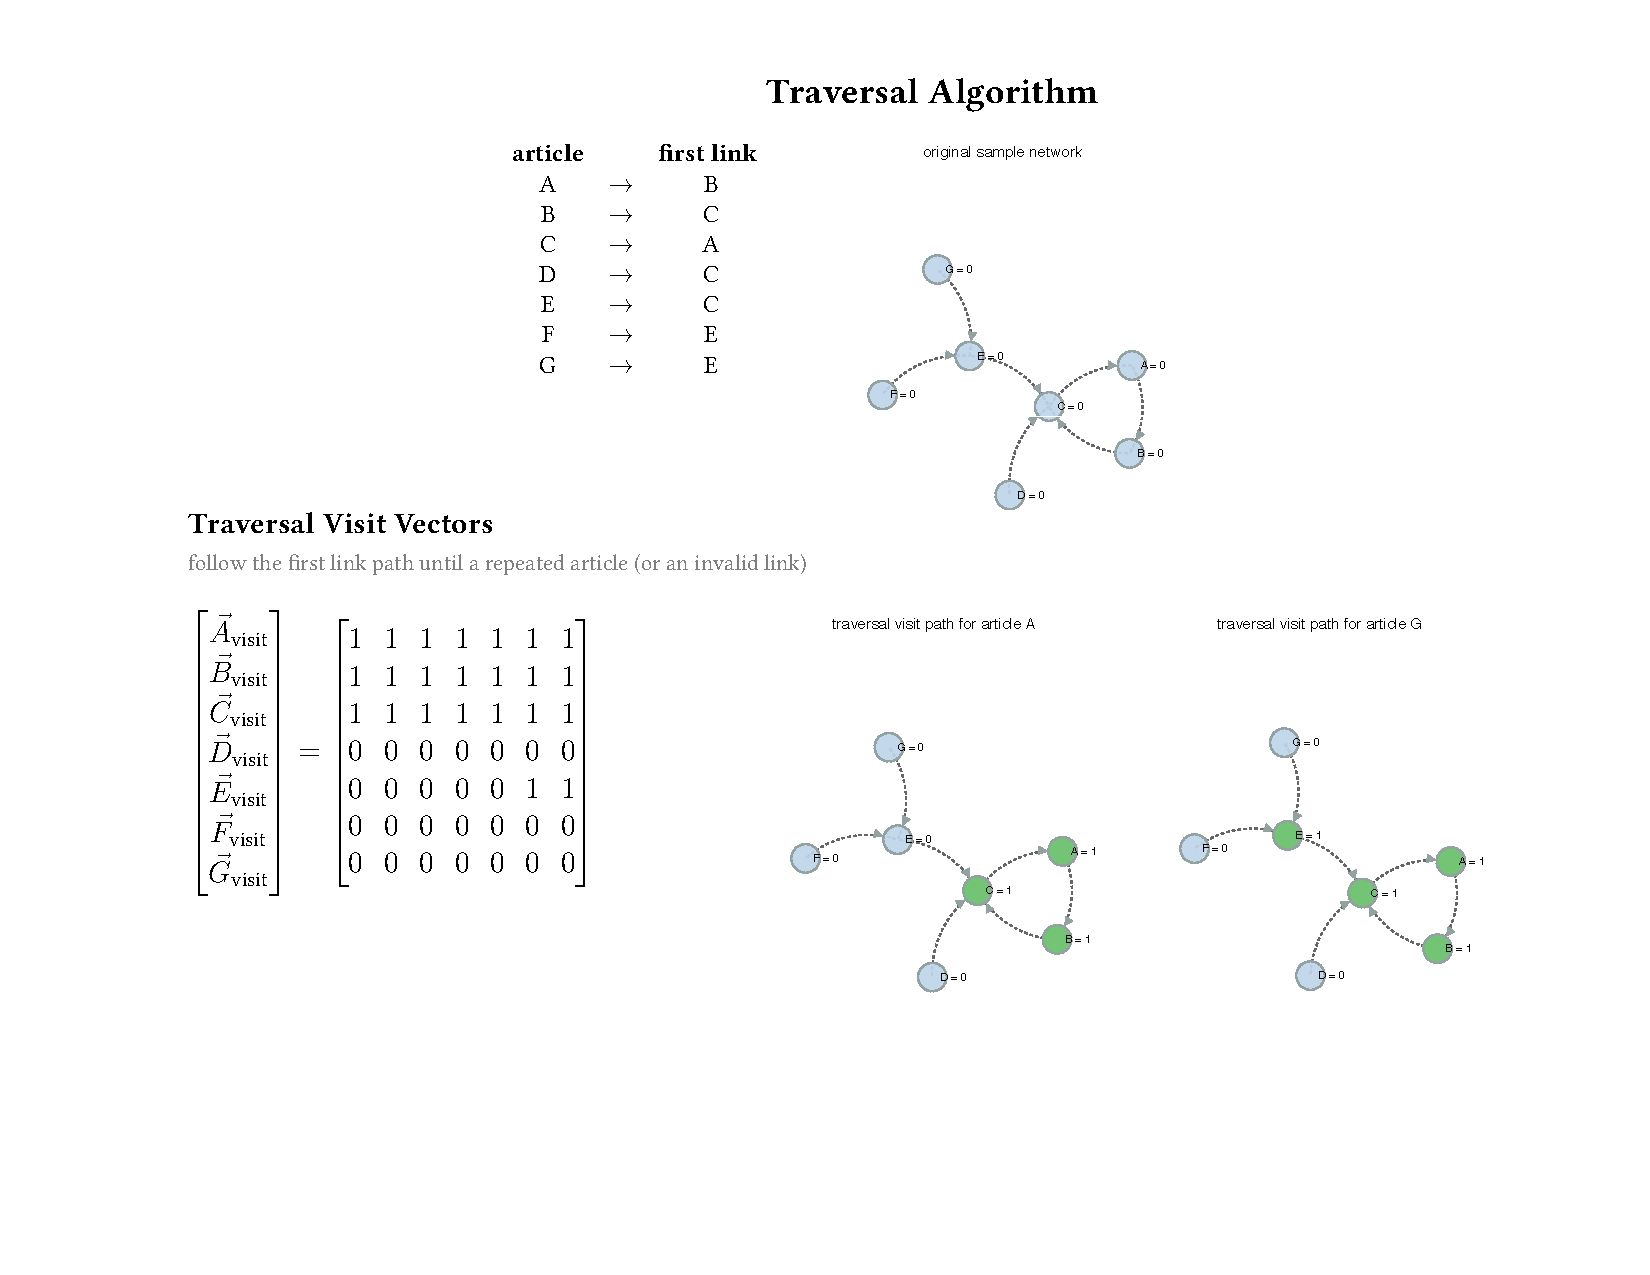
\includegraphics[width=\textwidth]{graphics/traversal_visit_algo_figure.pdf}  
  \caption{
    \textbf{Traversal Visit Algorithm on a sample network.}
     The traversal visit vectors are an adjacency matrix for the paths through the network: the first column is indicates the path formed starting with article A. The number of traversal visits for article A is then the number of paths containing A or the sum of the first row in our matrix:
     $\sum_{i=1}^7 A_{\text{visit, i}} = 7$.
  }
  \label{fig:Traversal Visits}
\end{figure*}

Applying a similar concept with  
varying starting articles, we form 
paths through the FLN moving from one article to the next.
A path in the FLN connects a group of articles, allowing us to measure how two articles relate,
even if the articles are not directly linked. 
Path-connected articles express a flow of concepts.
The notion of paths allows us to map not only which articles link directly to "Philosophy" 
for example, but also which ideas flow to "Philosophy":
path-connected articles to "Philosophy."
The method is order agnostic with respect to which articles are selected first. As long as each article is selected eventually, the resulting metrics are equivalent.
Starting at each article, we construct a path through the FLN, 
ultimately mapping a flow of connections among articles.

In a novel approach, we use the notion of a path through the FLN to describe 
the structure of the FLN as a flow relating ideas. 
Grounded in the dynamics of river networks,
\cite{geo_basins}
we characterize features of the FLN as a flow through First Links.
Previous studies have used flow to characterize the structure of river networks
\cite{dodds} and describe the organization of food systems as transportation networks
\cite{food_webs}.
With paths to mark flow through the FLN, we develop new metrics to 
gauge the accumulation of references, 
the length of the path relating articles, and the influence a particular
article exerts in shaping the flow of links through the FLN.


Our goal is to map the flow of First Links by following the paths of First Links 
starting at each article. 
Since a path reveals how the ideas in one article may eventually be 
anchored in another, the first metric we develop quantifies the accumulation of First Links.
The algorithm begins by selecting an article, then traversing the path formed
by following the First Links. Each time a First Link references an article, we increment a count
associated with the article. 
We continue until the First Link is repeated or is invalid---defined here to mean outside of Wikipedia.
We select a second article and repeat the process until we have 
constructed a path for each article in the network. We call the resulting count for each article the number of {\it traversal visits}. The number of traversal visits of an article 
measures the number of references flowing to the ideas in the article. 

\begin{figure}[tp!]
  \centering	
  \includegraphics[width=\columnwidth]{graphics/traversal_funnel_algo_figure.pdf}
  \caption{
    \textbf{Traversal Funnel Algorithm on a sample network.}
  The algorithm for traversal funnels is identical to the previous algorithm for traversal visits with one alteration: the path ends at the start of a cycle to distinguish articles directing a path into a cycle from articles that simply happen to be in a highly traversed path. We can construct similar vectors by considering each path through the network, measuring traversal funnels for a particular article as the sum of the entries in its corresponding row. For example
  the number of traversal funnels for article $E$ is 
  $\sum_{i=1}^7 E_{\text{funnel, i}} = 2$.}
  \label{fig:Traversal Funnels}

\end{figure}

We can characterize the paths in the FLN as a matrix with each column corresponding to a path. In our sample network 
(see figure~\ref{fig:Traversal Visits}), the path starting at article A is the 
first column in the traversal vists matrix. 
An entry of $1$ indicates the path contains a given article and 
$0$ indicates the path doesn't. The columns identify the starting article of the path. 
For example, the second column corresponds to the path starting at article B. 
To compute the number traversal visits for article A we sum the corresponding row in our matrix.
The total is the number of paths containing article A. 
Analogous to the flow 
in a river network, traversal visits measure the accumulation of water at point A. 
By constructing a traversal visits matrix, we can similarly compute the number of traversal 
visits by summing along the corresponding row. The traversal visits matrix for 
Wikipedia consists of 121 million entries to account for each path through the FLN. 
We measure the accumulation of First Link references by summing the corresponding row for the 
article of interest.


In addition to accumulation, the traversal visits algorithm creates paths 
which uncover depth in the FLN. 
By measuring the number of First Links between
two articles, we get an additional piece of information we call 
{\it path length.} We can compute the length of a path by summing 
along a column in our traversal visits matrix. 
The path length describes how closely related ideas are, gauging the FLN's depth.
The greater the number of First Links separating two articles, the greater the number of ideas needed to relate their corresponding ideas. Although
"Train" is related to "Economics" for example, there are several articles
bridging the connection:
"Train" is more specifically related to transportation, whose object
is often goods. Goods are one of the fundamental objects of study in Economics.
Described in links, this relationship is captured by a relatedness of $4$ 
First Links ultimately connecting "Train" to "Economics." 
We can examine path length as a relative measure of how closely connected ideas
may be, but also as an aggregate measure describing the overall separation or 
connectedness in the FLN.
We can characterize whether ideas are closely connected by a handful of links, 
many, or whether a more nuanced organization exists. 


One possible path through the FLN is a {\it cycle} or a group of articles 
linking to one another inside a loop. In our sample network 
(see figure~\ref{fig:Traversal Visits}) 
a cycle exists among nodes A, B, and C. 
Since node C links back to the starting node A, the path starting at node A forms a {\it 3-cycle}. 
By recording the history of the articles along a path in the FLN, we can identify
the types of cycle structures within the FLN. Furthermore, since each article 
has an associated traversal visit count, we can rank cycles by 
the number of references directed towards a cycle. 
We can also form and rank {\it basins} in the network by identifying groups of 
path-connected articles, not necessarily forming a perfect cycle.
A basin connects a group of articles and identifies the paths 
to a particular article.
By identifying basins and cycles, we pinpoint groups of closely related articles.


While traversal visits measure accumulation, each article's First Link also 
influences the shape of the FLN. 
At a large point of accumulation, a single article's First Link 
can exert great influence over the shape of the FLN by directing many
references on a particular path. To distinguish between an article 
that simply happened to fall within a cycle from an article funneling 
many First Links, we develop a second metric called {\it traversal funnels}.

To measure traversal funnels, we traverse the FLN in the same manner as we 
did for traversal visits, but end a path once we enter a cycle.
We are then able to distinguish between an article related to many other ideas
only by virtue of its place in a cycle, from an article exerting influence over where the First Links flow. 
An article with a large number of traversal funnels directs many references
towards a particular cycle. In our sample network 
(see figure~\ref{fig:Traversal Funnels}) article C 
directs the flow of links towards the 3-cycle, while articles A and B are 
recipients of the flow---without exerting any direct influence themselves. 
While articles A, B, and C all have the same number of traversal visits, 
article C has 4 traversal funnels (A and B have none). By incrementing the count of 
First Link references on paths only up to a cycle, we can identifying which articles
exert the greatest influence over the FLN's structure.

By studying the FLN not only as collection of directly linked pairs of articles, but
as a flow, 
we build a powerful arsenal of information with which to study the FLN. 
From accumulated references, cycles and basins to influence, we can measure how the many articles in Wikipedia are organized and related.





\section{Discoveries}

\subsection{Degree Distribution}

\begin{figure}[tp!]
  \centering	
  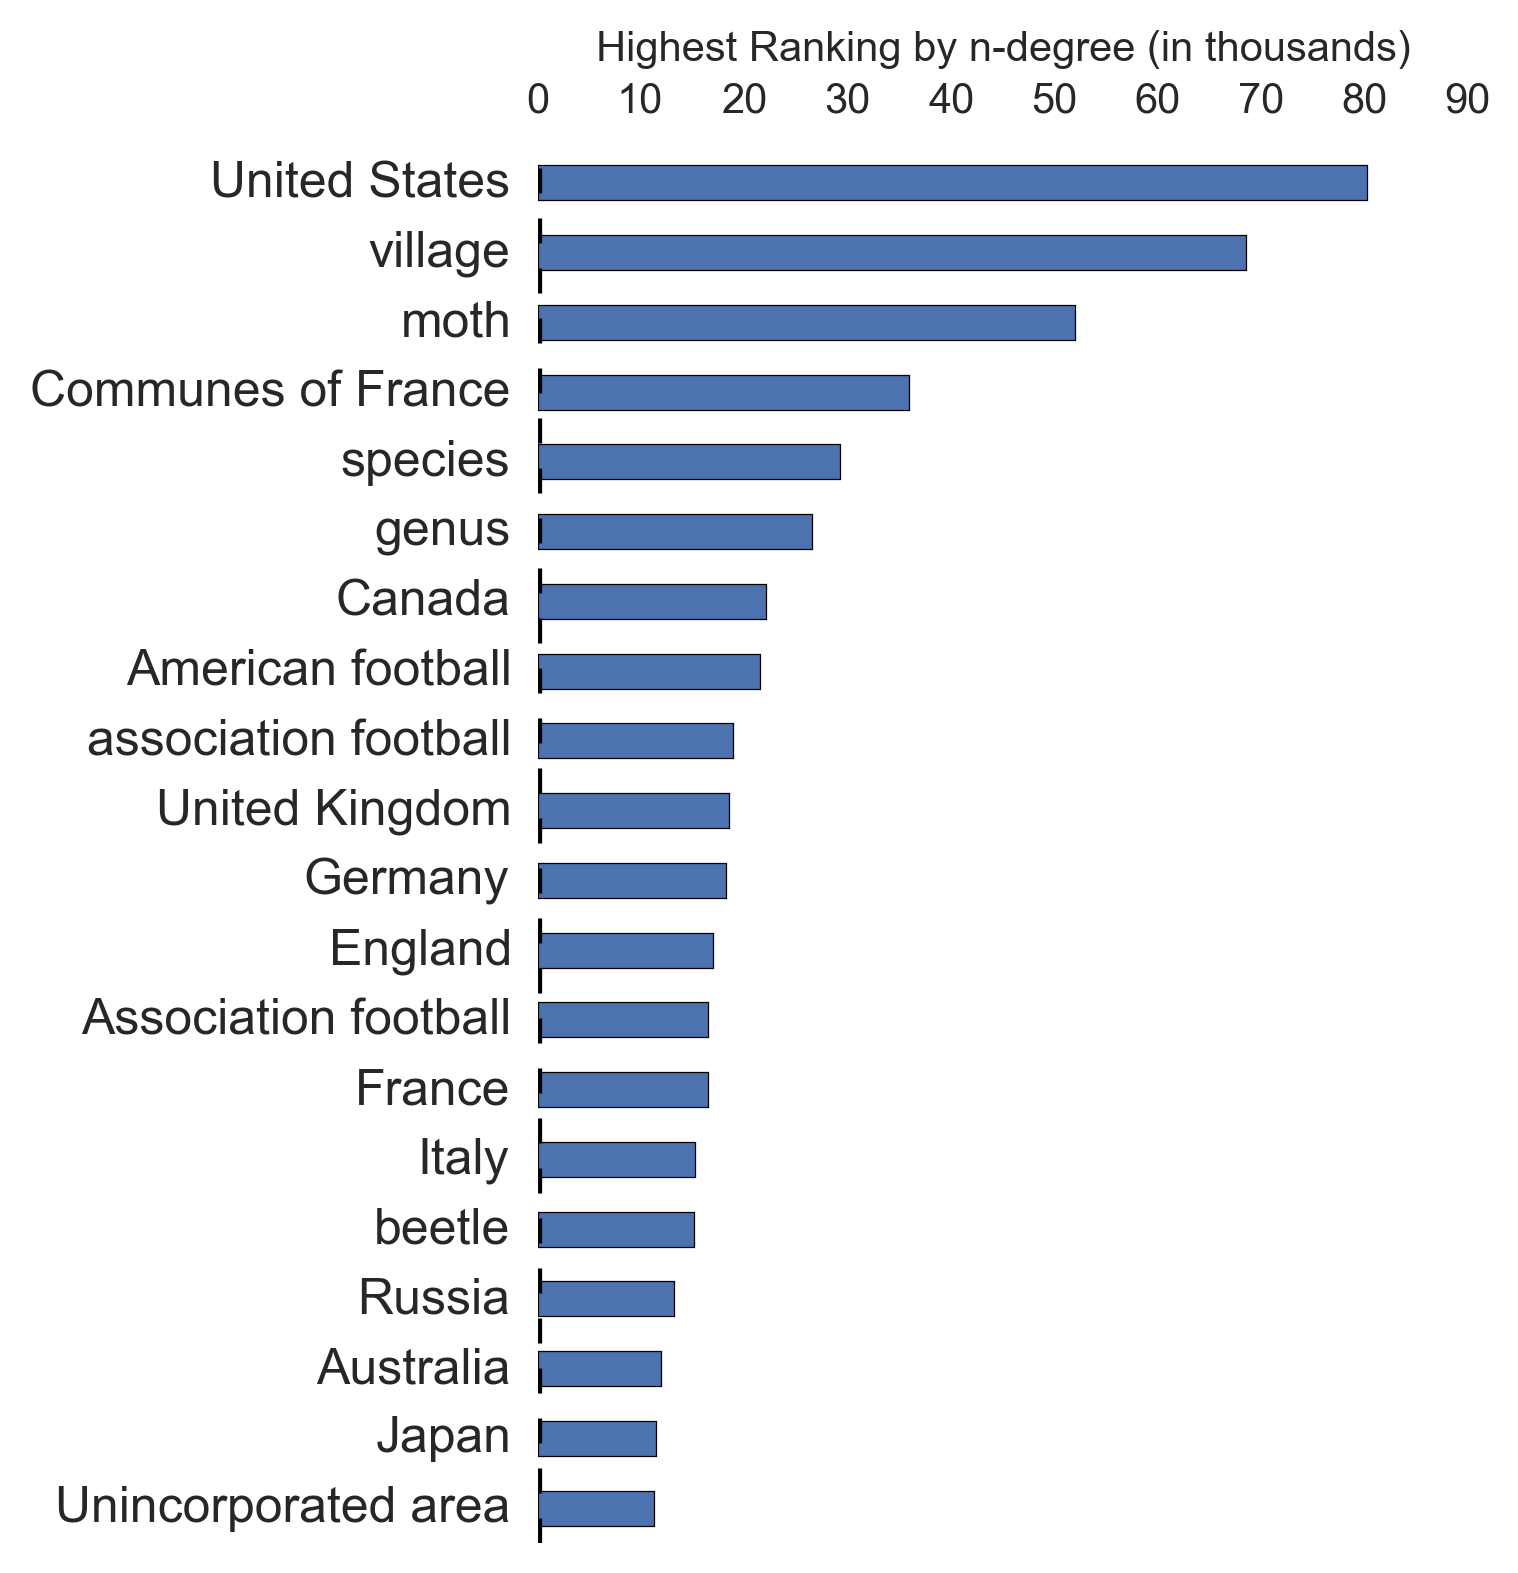
\includegraphics[width=\columnwidth]{graphics/articles_ndegree.png}
  \caption{
    \textbf{Highest Ranking Articles by indegree.}
  }
  We rank each article by the number of direct First Links to the article (indegree). The highest-ranking articles tend to represent abstraction for concepts
  comprised of various facets.
  \label{fig:ndegree list}
\end{figure}

We identify the set of First Links directly referencing a particular article 
by studying indegree in the FLN.
A higher indegree suggests more authors found the ideas in the article 
pertinent to reference. 
We rank all 11 million articles by indegree to find 
the "United States" with 80,249 direct First Links as the most referenced
Wikipedia article 
(see figure~\ref{fig:ndegree list}). 
Other high-ranking articles
include foundational abstract concepts such as "village," "species,"; 
sports associations such as "American Football," "Association Football"; 
and developed nations such as "France," "Japan," "Russia," "Australia," and 
the "Netherlands." These high ranking articles are useful abstractions: nations
describe a collection of individuals with a common culture, language, or 
geographical proximity; sports teams describe an ever changing collection of 
sports players often associated with a cultural identity or a geographical 
region. 
Since abstractions such as nations and teams are inherently comprised
of many parts, authors reference the abstraction when describing a part.
In describing the New England Patriots or the New York Giants
for example, "American Football" is the natural abstraction, which 
anchors many specific teams.

"Philosophy" and other philosophical concepts
are not among the highest-ranking articles by indegree.
"Philosophy" has an indegree of 581, with direct First Links from articles about Philosophers and areas of Philosophy: "Existentialism and Humanism," "Predeterminism," "Synoptic Philosophy,"Qualia," "Dorothy Emmet," and "Christopher W. Morris."
While many articles accumulate at "Philosophy" (see the coming traversal visits discussion), 
the accumulation is not the 
result of many articles directly referencing "Philosophy." 
Instead, the accumulation of First Links, as we argue in our 
discussion of traversal visits, flows towards Philosophy as the 
ultimate anchor when generalizing from specific articles to broader notions.

\begin{figure}[tp!]
  \centering	
  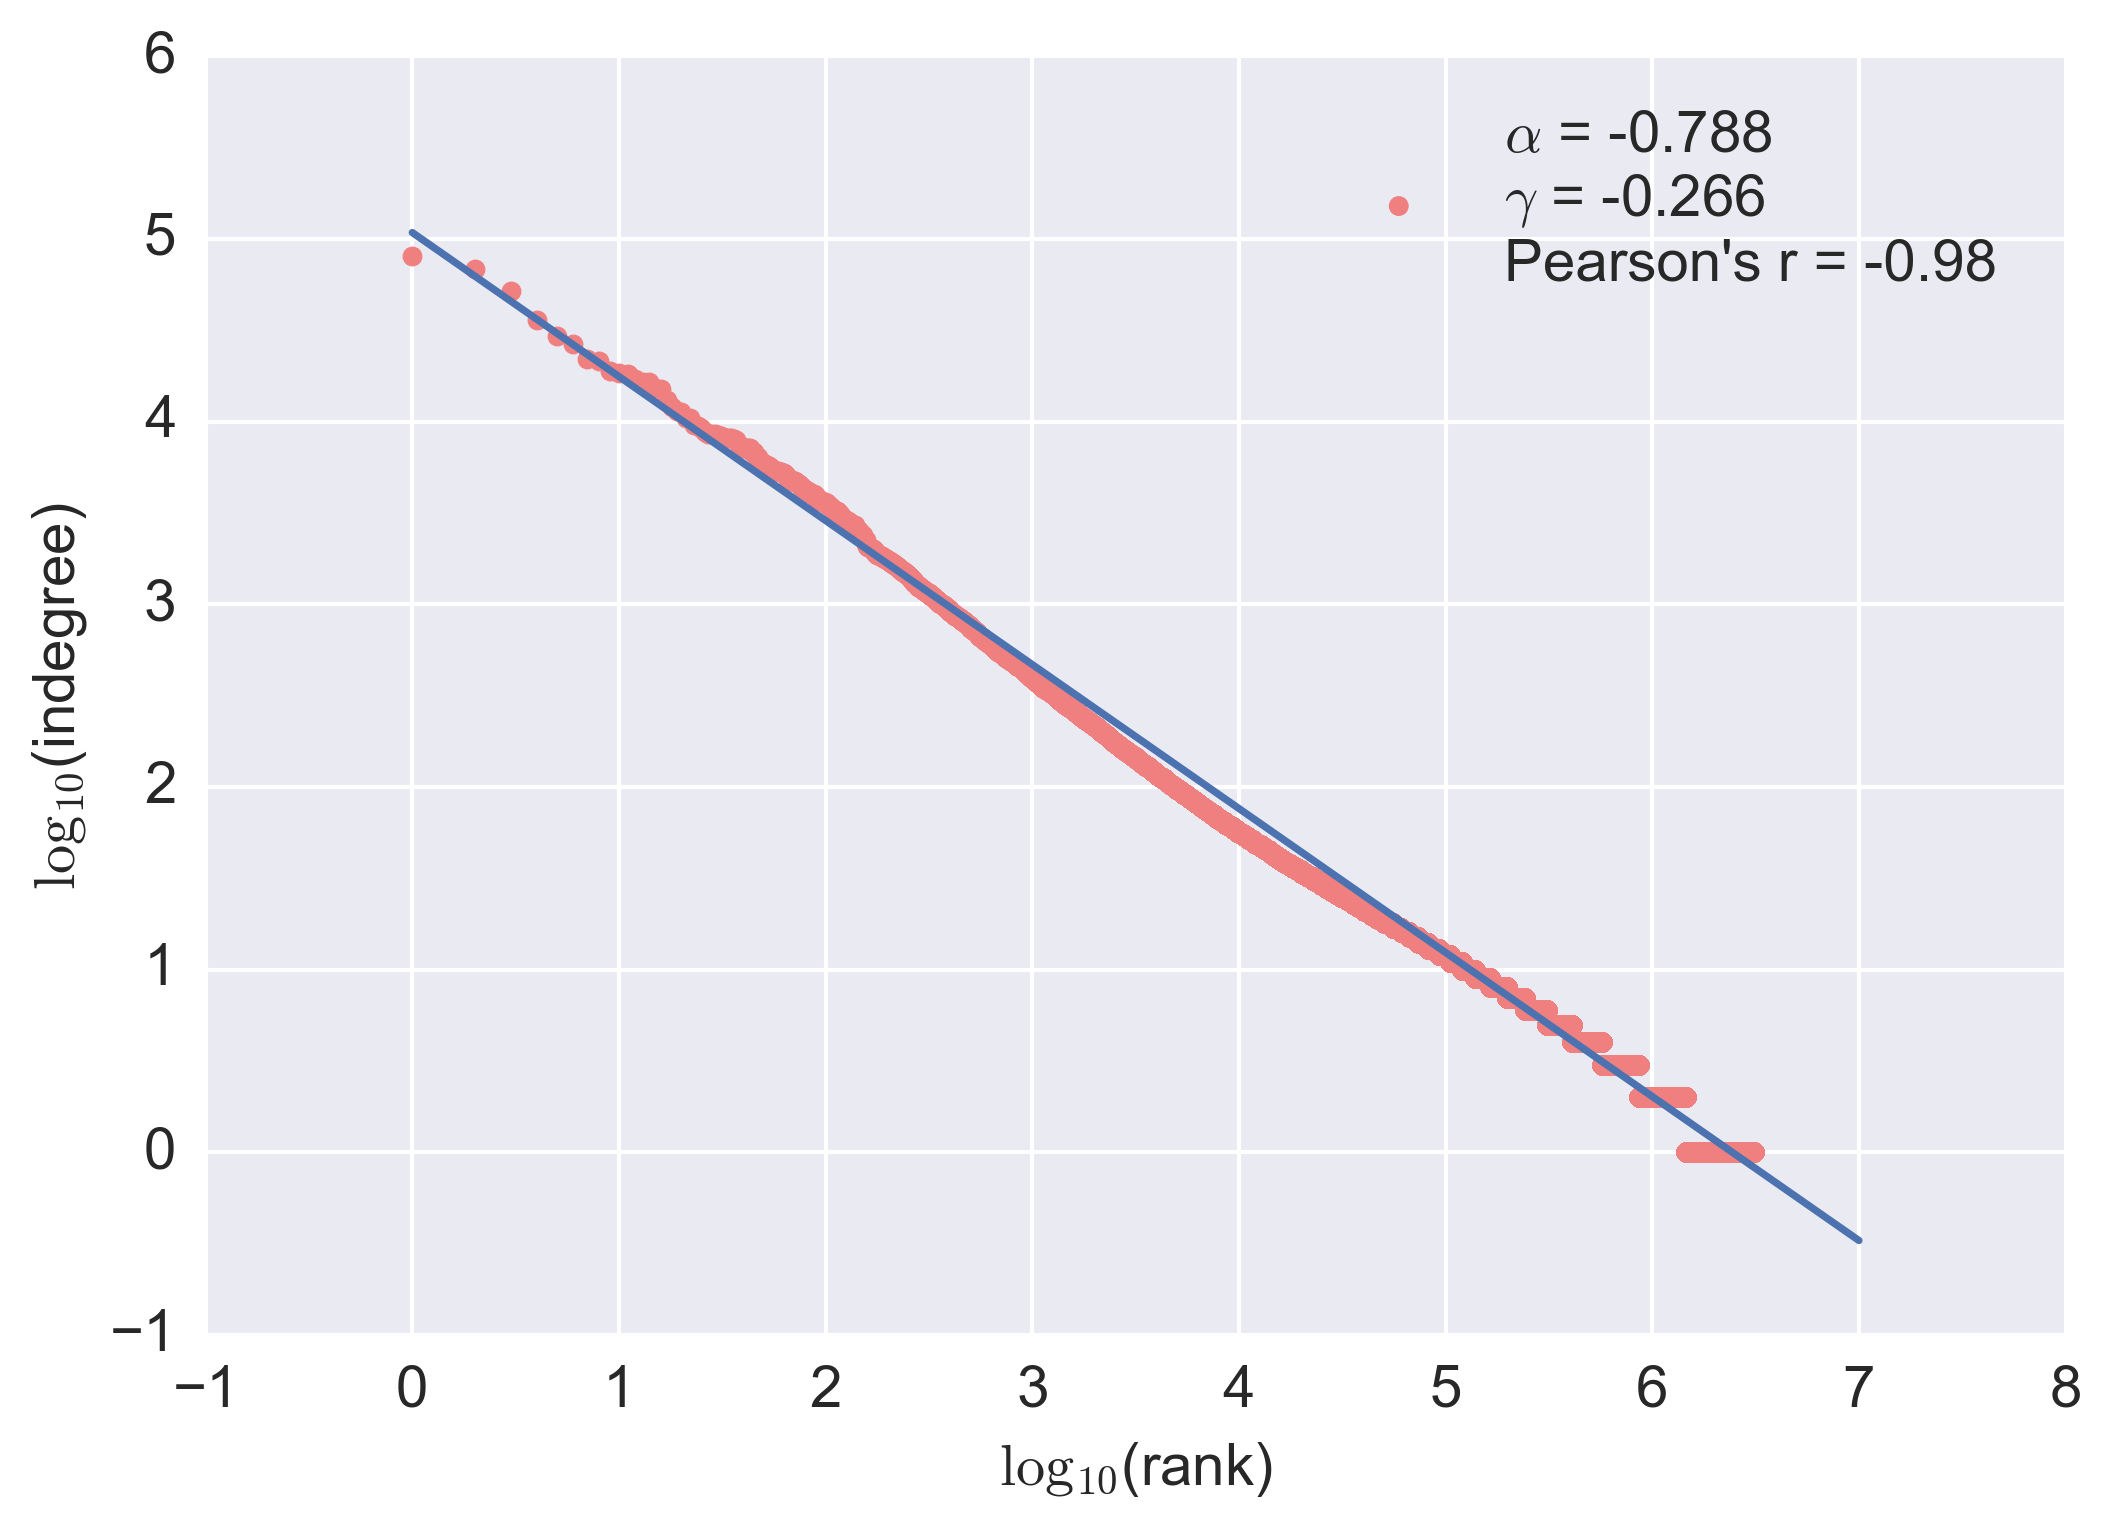
\includegraphics[width=\columnwidth]{graphics/ndegree_loglog.png}
  \caption{
    \textbf{FLN Degree Distribution.}
  }
  We construct a log-log plot and fit our results with a linear model. The result is a 
  an excellent fit with r = -0.98, yielding a power law exponent of -0.79. 
  The distribution appears to be scale free.
  \label{fig:degree distribution}
\end{figure}

The FLN's indegree exhibits a scale-free distribution where a few articles 
receive most direct first references; most articles receive few or none.
The average indegree for all 11 million articles is 3.6 direct First Links with a standard deviation of 89.5 links.
Only 4,826 articles have more than 100 direct First Links and $75\%$ of articles
have fewer than 9. 
When fit with a linear model on a log-log scale (log(rank) versus log(indegree)), 
the model's r value is $-0.98$ suggesting a strong log-log linear fit 
with a power law exponent of $-0.79$.\\

\centerline{***}

Beyond indegree, we develop the notion of a path to describe the structure of the FLN as a 
flow relating ideas. We traverse every possible path through the FLN, taking 
$232$ million steps along the way.


\subsection{Depth of the FLN}

We first seek to describe the depth of the FLN: how many links does a 
connection of ideas span? We gauge the FLN's depth by 
measuring path length or the number of links traversed until a repeated or invalid link (one outside the FLN). 
We discover the longest path length is 365,
corresponding to the yearly calendar of Orthodox Liturgics.
Each day's Liturgics links to the next day's. On the last calendar day, the last article simply links back to January 1, forming a 365-cycle 
(see discussion of cycles).
We also find similarly lengthy paths following the evolution of a place or topic through time: 
"1953 in Scotland" or "1560s Architecture", with articles sequentially proceeding by year, decade or era.
The longest paths connect temporally organized ideas.

\begin{figure}[tp!]
  \centering	
  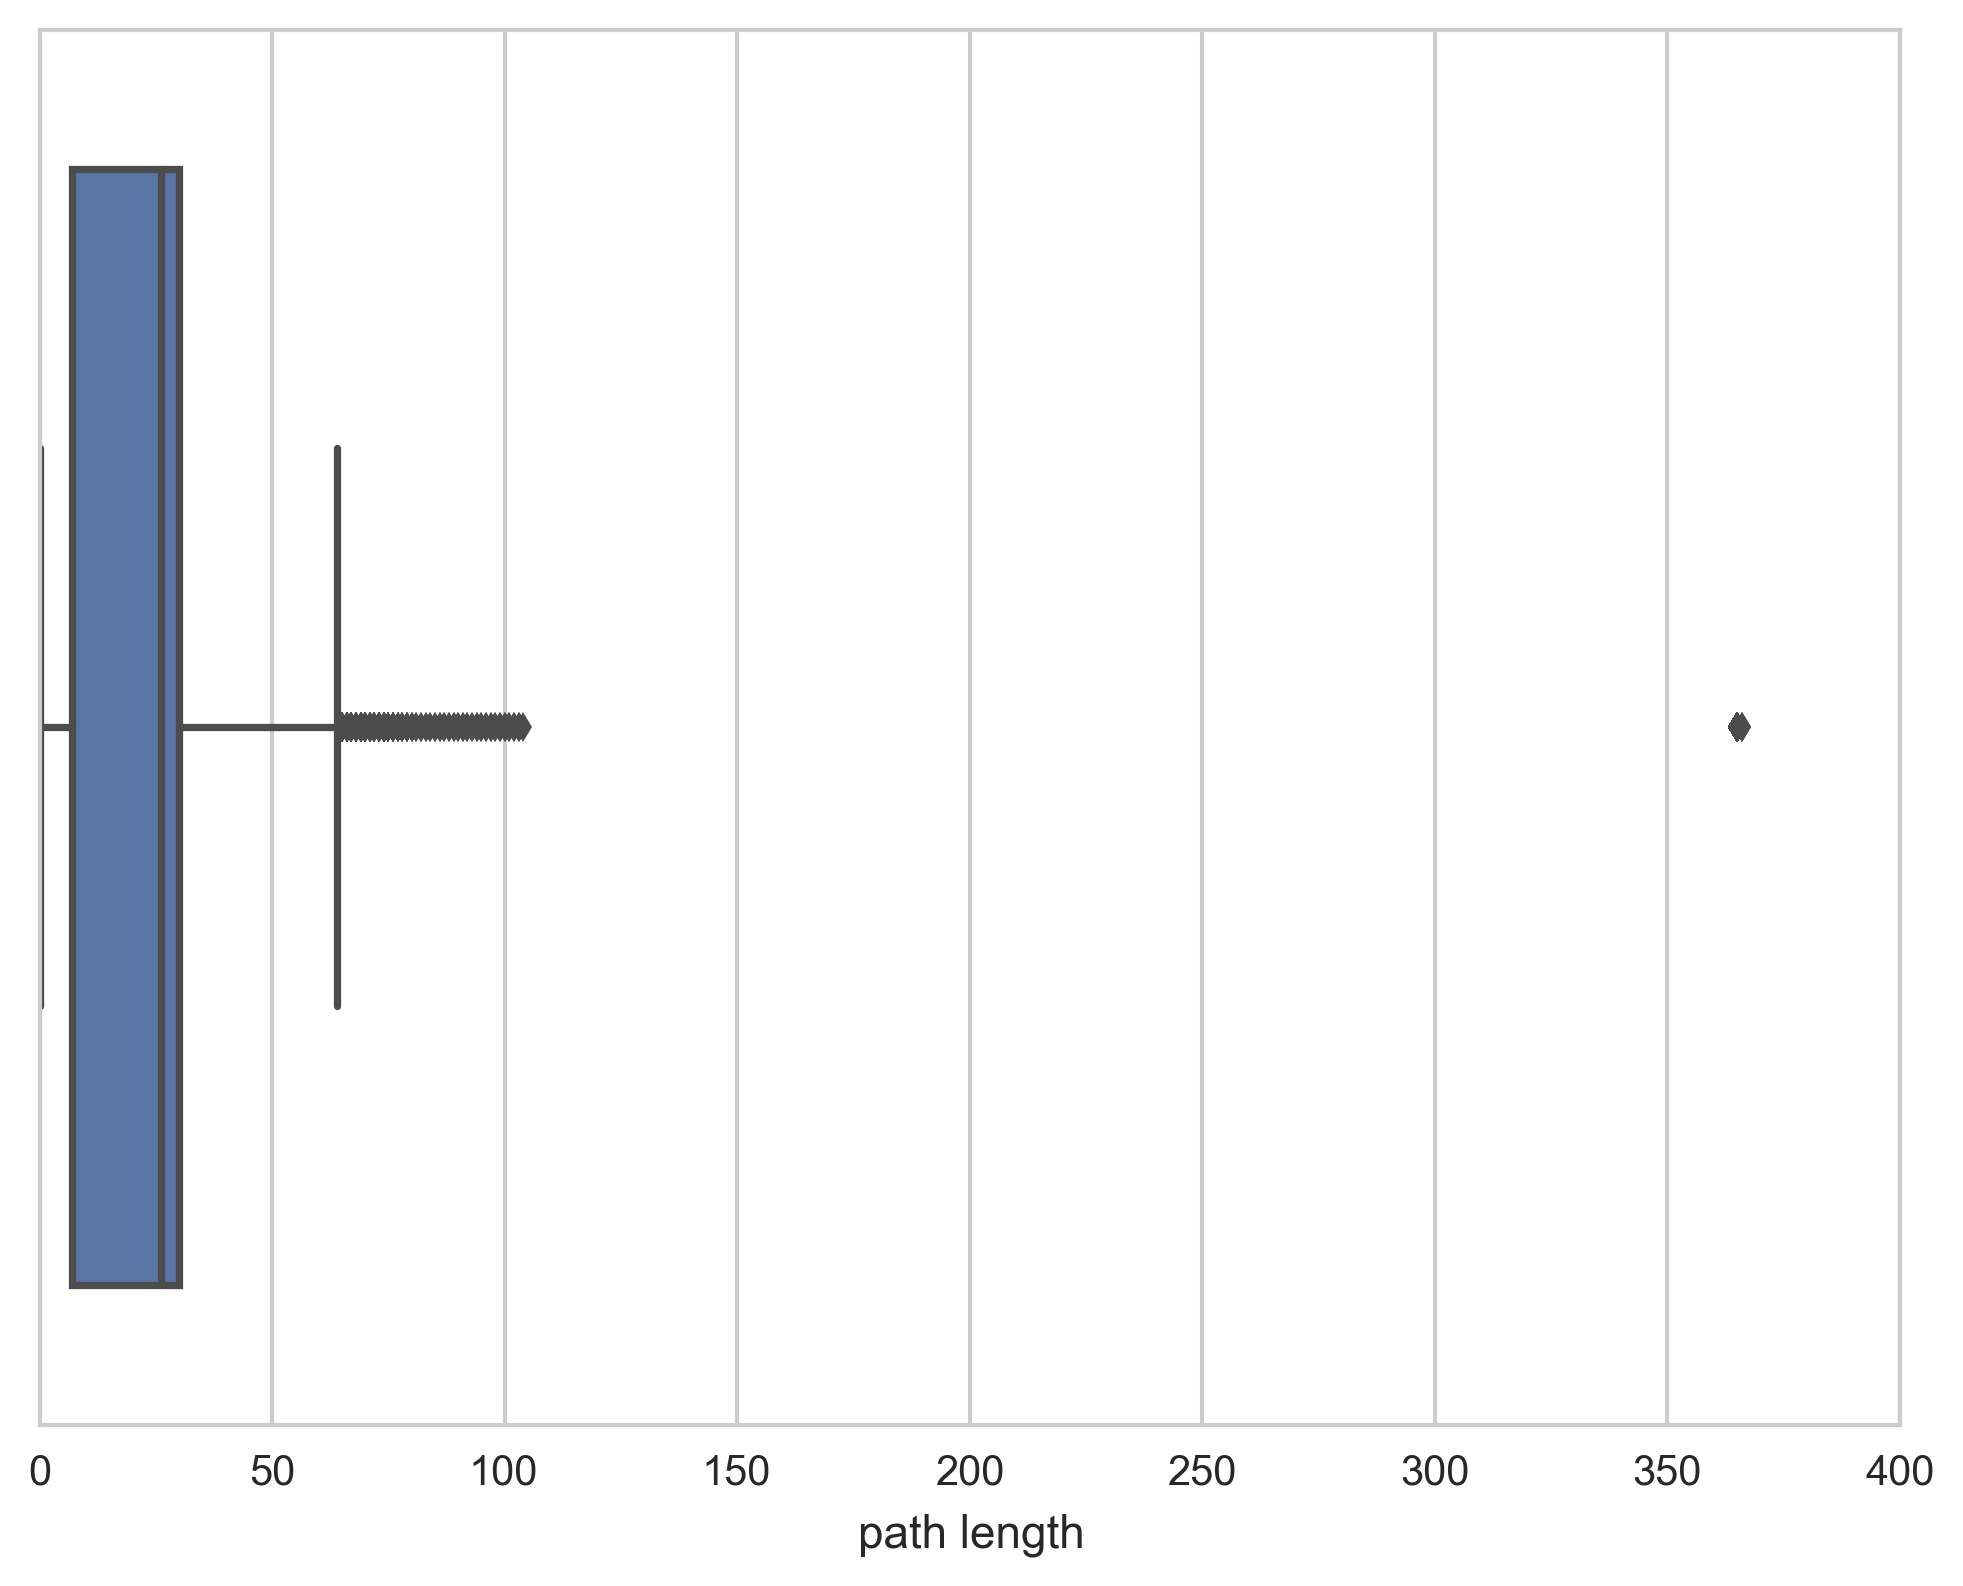
\includegraphics[width=\columnwidth]{graphics/path_lengths_boxplot.png}
  \caption{
    \textbf{Path Length Distribution.}
  }
  The median network depth measured by the number of First Links in a path
  is 29. The 365 cycle for "Orthodox" liturgics is the outlier to the right, while
  other historical articles about "Scotland," "UK" and so on are slightly outside
  the third quartile. More than $75\%$ of articles have path lengths between 
  $0$ and $50$ links.

  \label{fig:Path Length Distribution}
\end{figure}

Of the 11 million articles, 5.5 million had an invalid link or linked back to the same article, yielding a path length of zero. 
This roughly corresponds to the official number of articles on Wikipedia: 
$~4.7$ million as of November 2014---approximately half of the 11 million 
articles in the XML dump are redirects or disambiguations, not full articles.
The most common path length is 29, with an interquartile range of 4---path length
is typically between 26 and 29 articles.
The median path length far exceeds the popular 6-degrees of separation (see for 
example the average number of academic publications separating scholars 
\cite{six_degrees}), indicating a greater network depth.
The network's depth suggests ideas are not related in small independent clusters. 
Instead the many diverse ideas fit together in long-chained connections.
As a distribution, more than $75\%$ of articles have a path length below 
$50$ First Links 
while a few temporally organized paths exceed 50 links 
(see figure~\ref{fig:Path Length Distribution}). 

How can we characterize the flow of ideas along a path? Next, we develop 
a metric to gauge the accumulation of First Link references
and describe a pattern for how ideas flow through the FLN.




\subsection{Traversal Visits}

We follow every possible path through the network, incrementing
the number of traversal visits for every First Link reference.
We generate a total of 232 million traversal visits.

As a distribution, the number traversal visits by article appears to be scale-free. 
The majority of articles have fewer than 30 traversal visits. 
First Link references accumulate at a few articles.
Specifically, $99.76\%$ of articles have fewer than $100$ traversal visits; nearly $80\%$ have none. 
Meanwhile, the highest ranking 30 articles have an extremely disproportionate number of traversal visits.

\begin{figure}[tp!]
  \centering	
  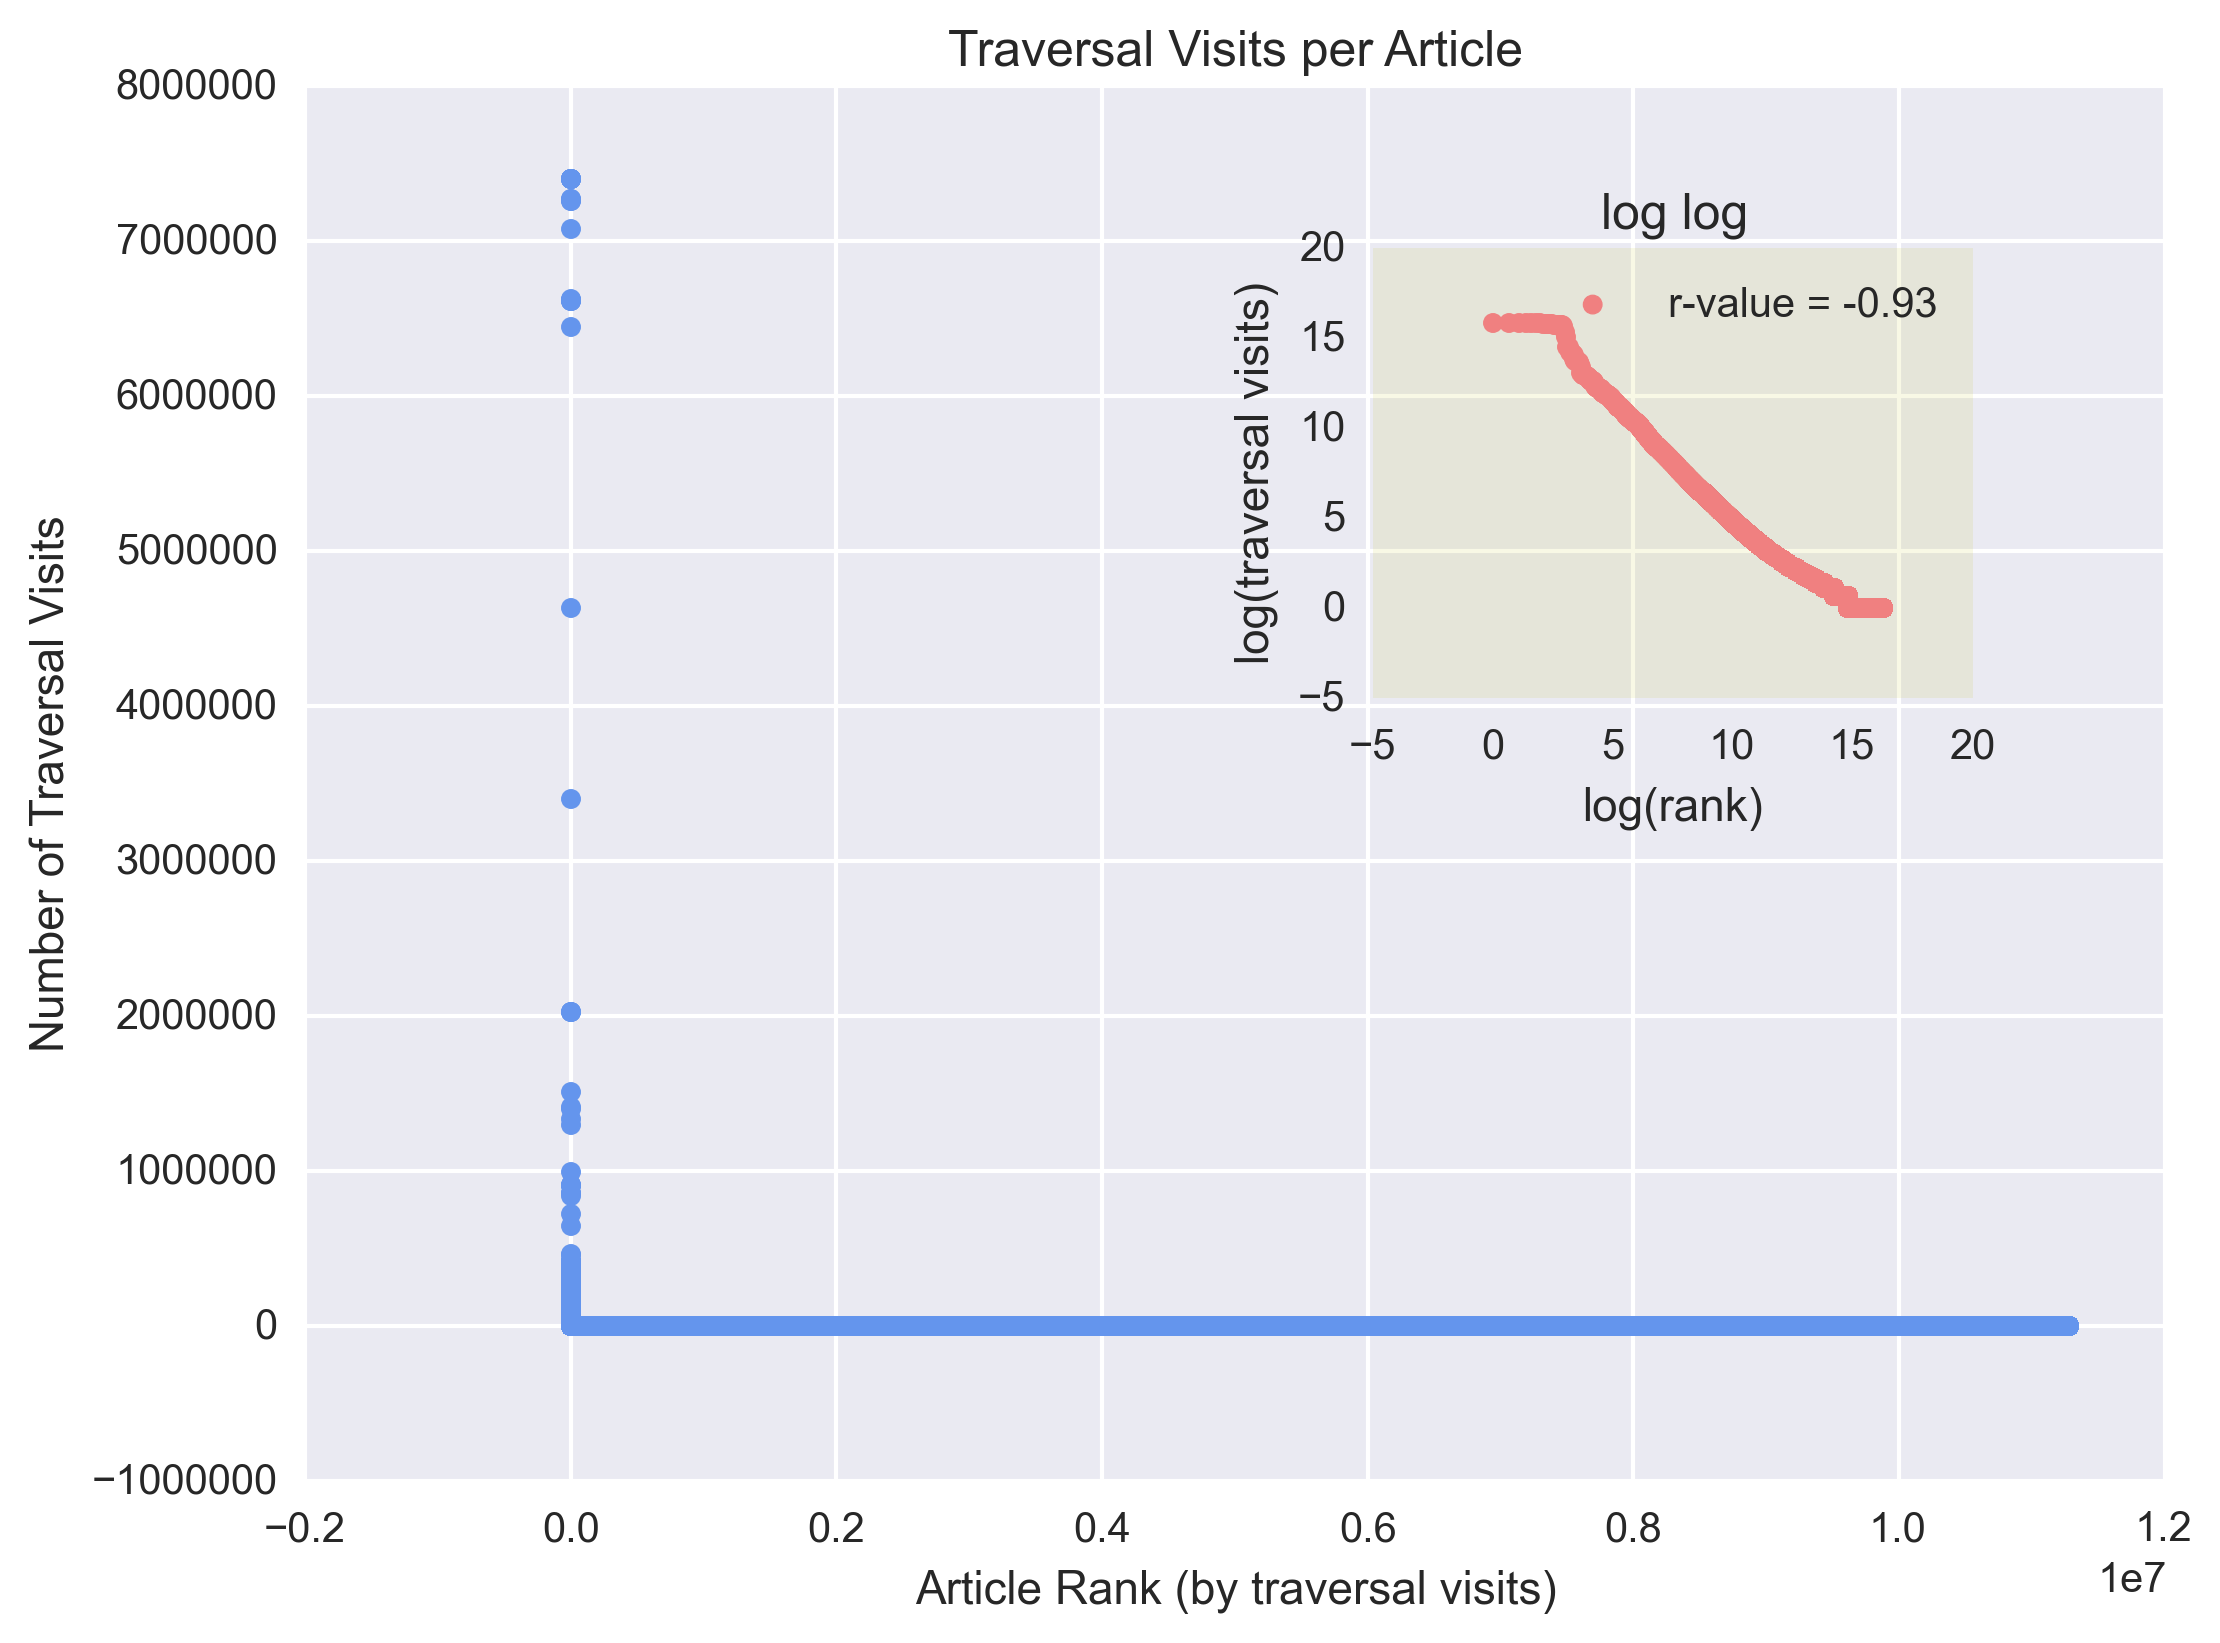
\includegraphics[width=\columnwidth]{graphics/traversals_per_article.png} 
  \caption{
    \textbf{Distribution of Traversal Visits.}
  }
  We fit the distribution to a linear log-log model by considering the log (base 10) transformed rank of each article against log (base 10) transformed the number of traversal visits. 
  The model explains $86\%$ of the variation in the data, yielding an r-value of $-0.93$ 
  and a power law exponent of $-0.64$. The horizontal flattening around the highest
  ranking articles is a result of the cyclic structure (see discussion on cycles).
  \label{fig:Distribution of Visits}

\end{figure}

To more accurately gauge the distribution, we construct a log-log plot of the entire dataset: log(traversal visits) against log(rank). 
We observe a strong linear fit, as is characteristic of scale-free networks, with an r-value of -.93 and 
a power-law exponent of $-0.636$. A handful of the highest ranking articles contain a disproportionate number of traversal visits, while most have none. The skew in the distribution is not terribly surprising when considering the heuristic of how the links flow: from specific to general. 


\begin{figure}[tp!]
  \centering	
  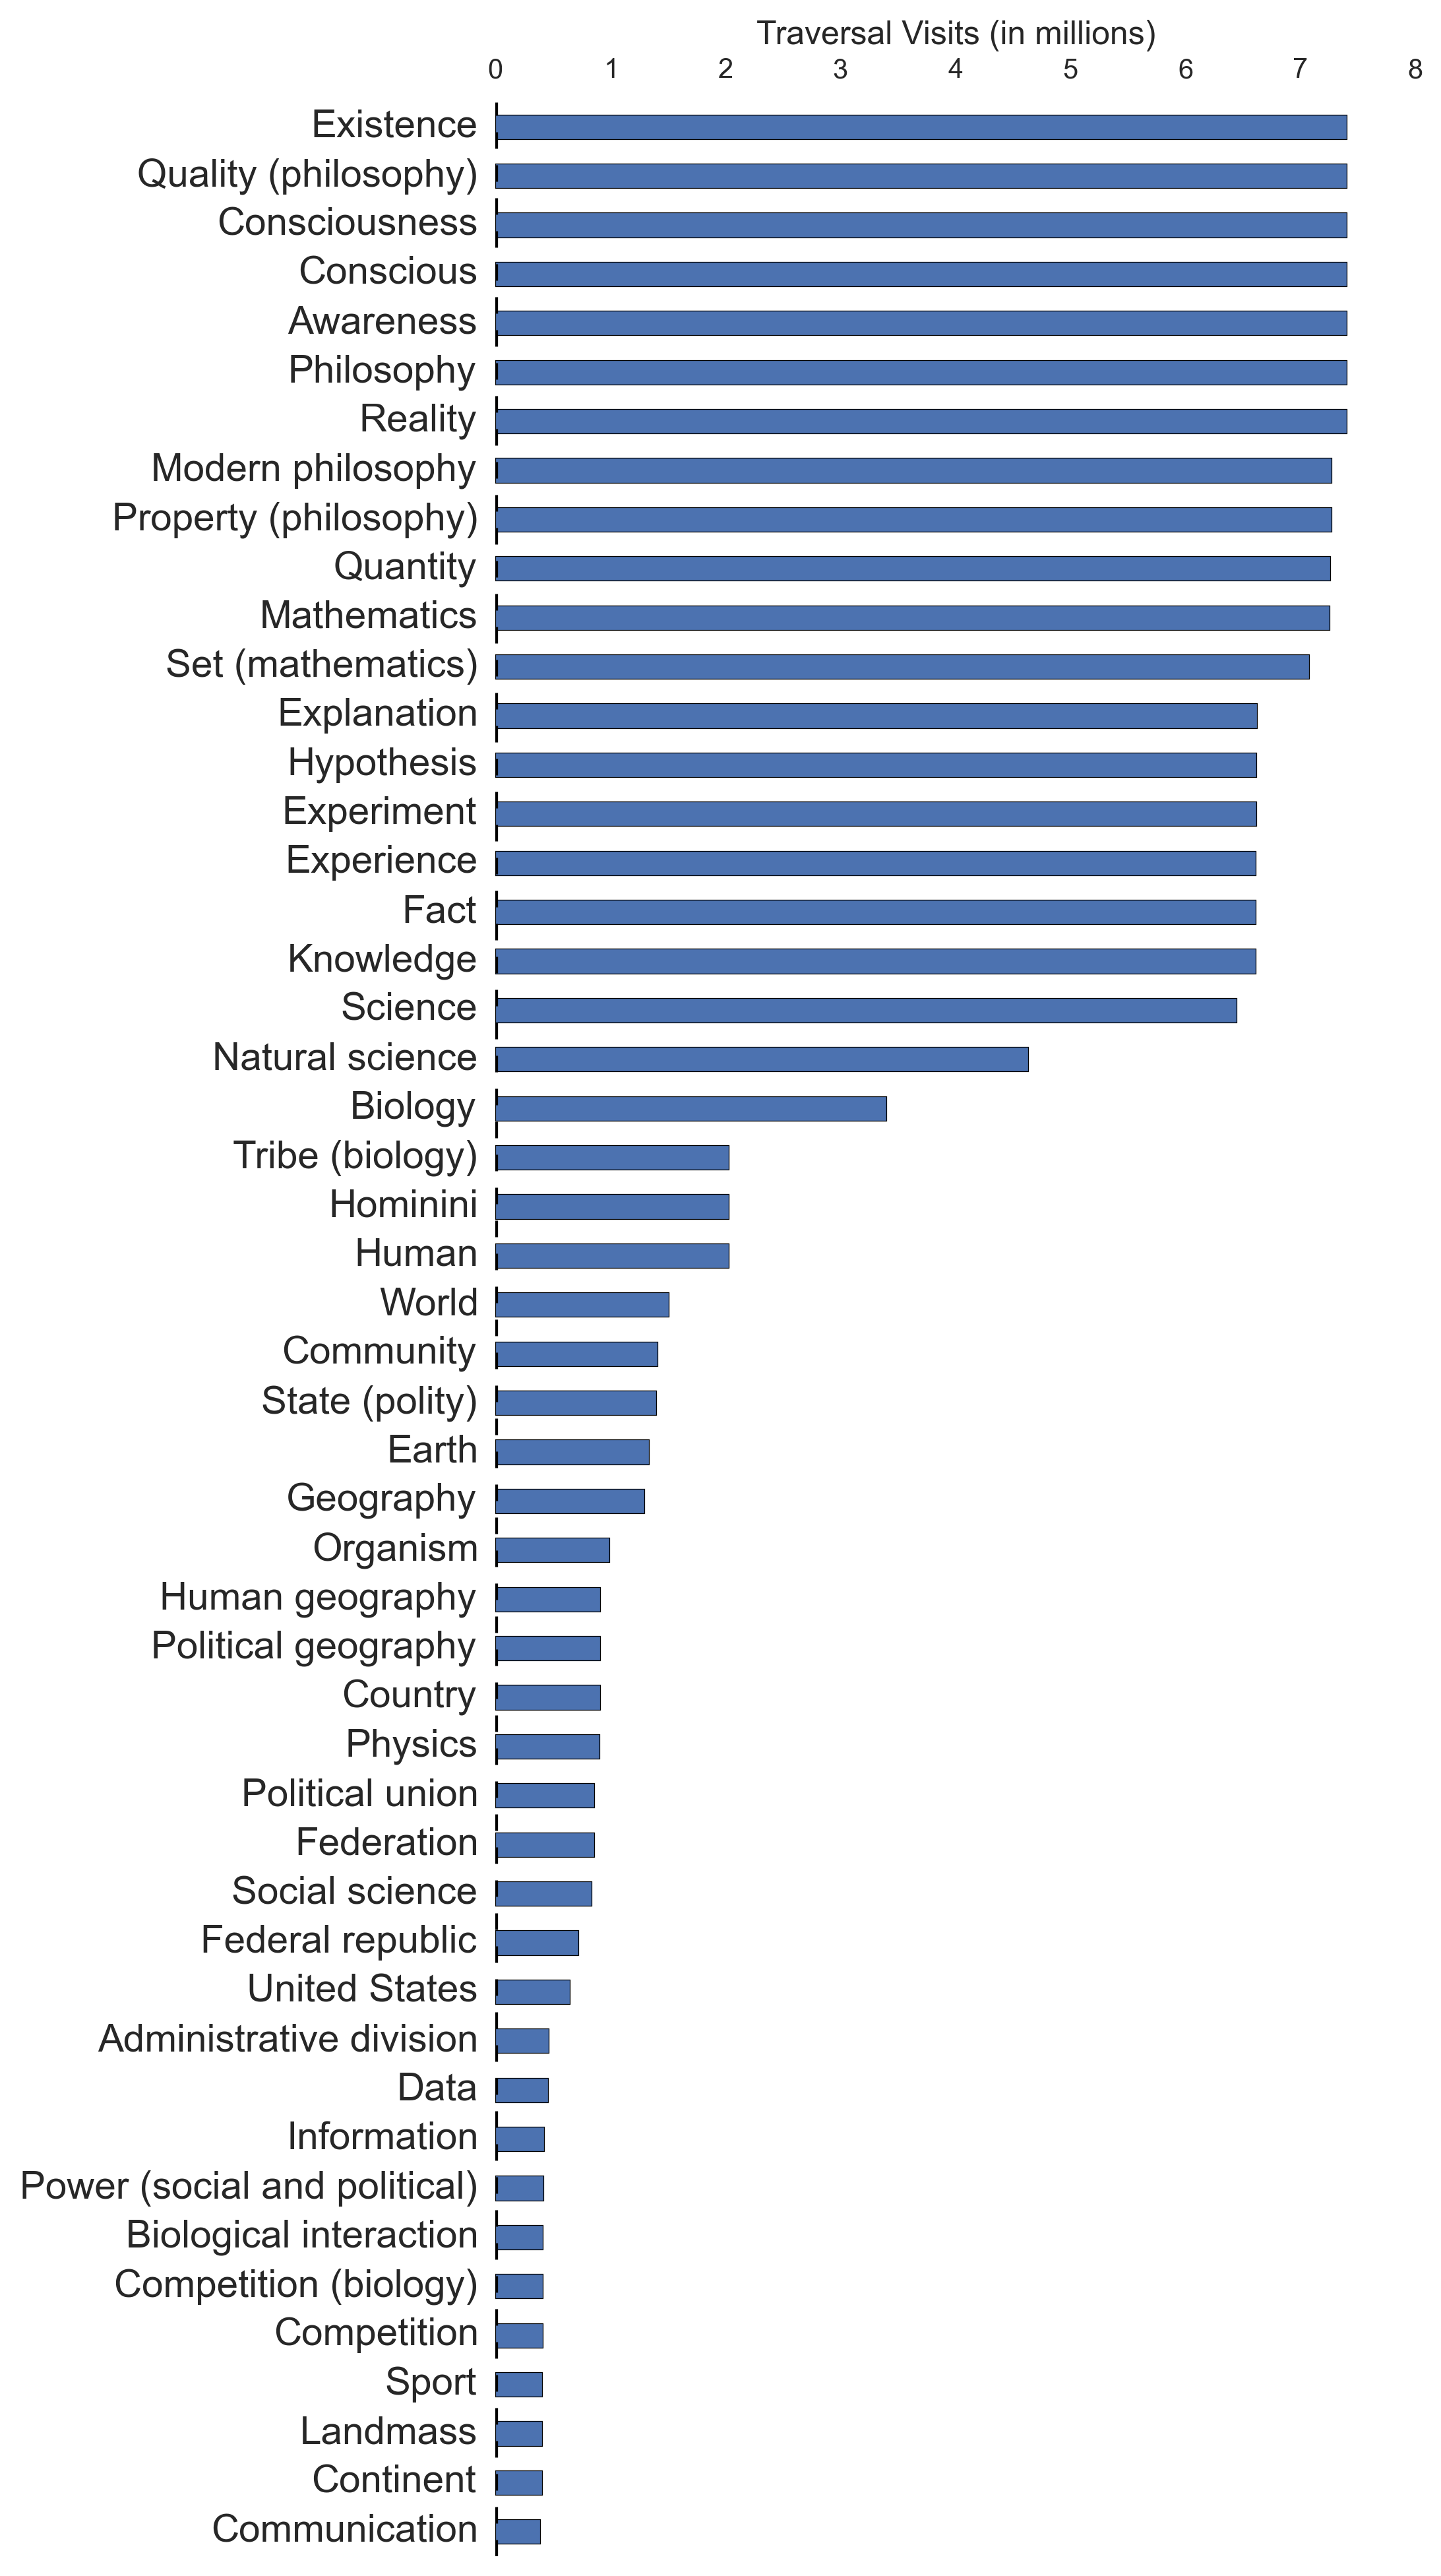
\includegraphics[width=\columnwidth]{graphics/articles_ranked.png}
  \caption{
    \textbf{Highest ranking articles by number of traversal visits.}
  }
  We compute the number of traversal visits for each article in the FLN (see 
  Traversal Algorithm section for details). In doing so, we can rank each article
  by the accumulation of First Links. Articles with a greater number of traversal visits
  mark greater points of First Link accumulation. The highest ranking articles by traversal visits reveal where the greatest accumulation occurs.
  \label{fig:highest visits}
\end{figure}


\subsubsection{A flow from general to specific}

The highest ranking articles by traversal visits are 
broad, global topics
(see figure~\ref{fig:highest visits}):
many are academic disciplines such as "Science," "Math," 
"Geography," "Philosophy," "Biology," and "Physics"; others are abstract fundamental concepts such as 
"Community", "State", "Earth", "Information", 
"Existence," "Communication", and "Power."
Since traversal visits measure the accumulation of First Link visits in Wikipedia, 
the highest ranking articles suggest First Links flow from specific to general articles. 
For example the flow of First Links for the "Banana" article begins at a very concrete
and specific topic, then flows towards progressively broader disciplines, eventually 
culminating at "Philosophy": "Banana" links to the broader category of "Fruit," which then links to 
"Botany," eventually "Biology," then "Science" and ultimately "Philosophy." 


\begin{figure}[tp!]
  \centering	
  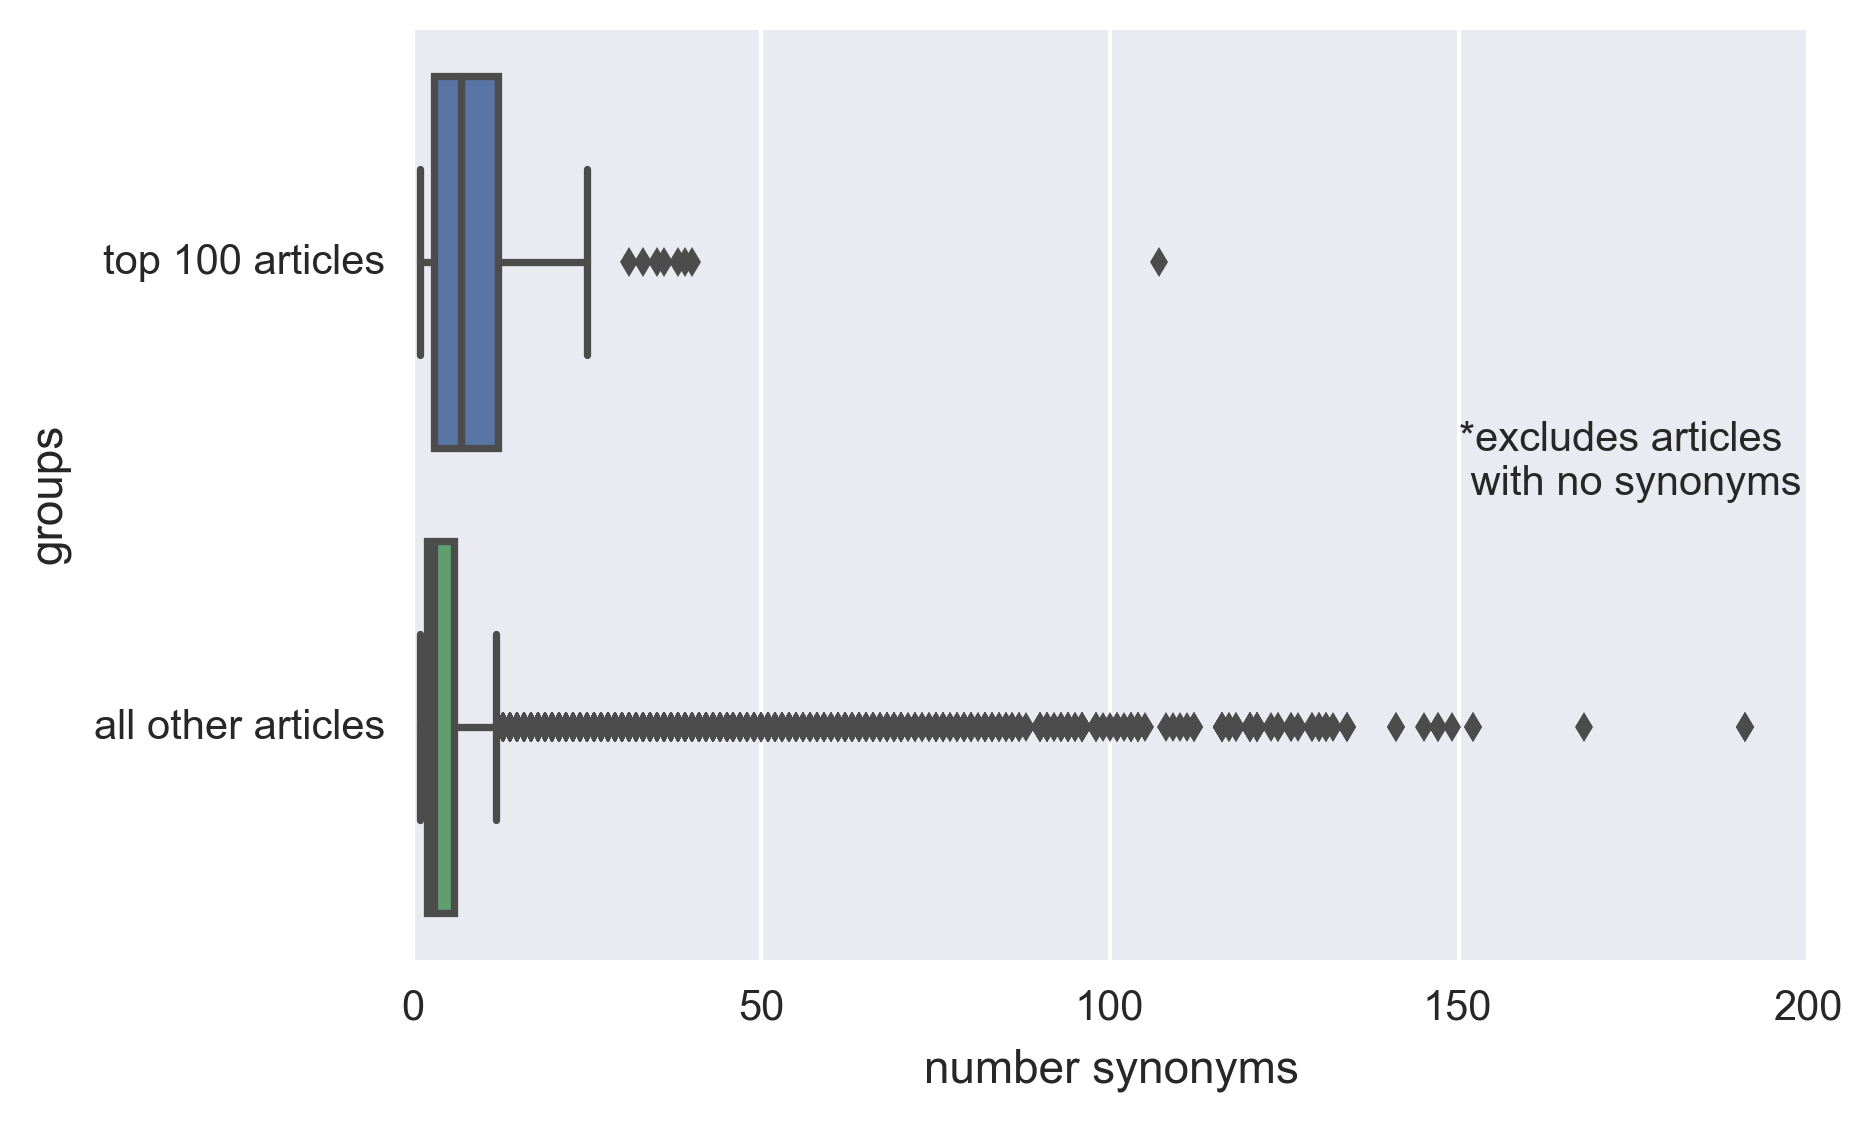
\includegraphics[width=\columnwidth]{graphics/synonyms.png}
  \caption{
    \textbf{Number of Synonyms for the highest-ranking articles.}
    We use WordNet (the largest lexical database for the English language)
    to identify the number of synonyms for an article's title. We compare 
    the distribution of synonyms of the highest-ranking 100 articles
    against all other Wikipedia articles (with the top 100 articles removed). As the distribution demonstrates
    the highest ranking concepts have more synonyms than other articles.
  }
  \label{fig:synonyms}
\end{figure}

To measure the specificity of an article, we identify the number of synonyms available for a word or topic. 
A  broader topic likely has many more synonyms relative to a specific, concrete topic. 
Banana has fewer synonyms than botanical for example. 
To quantify the observed flow, we measured the number of synonyms each title contained in WordNet---the largest lexical database of the English language 
\cite{wordnet}. 
We compare the highest ranking 100 articles against the all other Wikipedia articles, with the top 100 articles removed.
We find the highest ranking 100 articles have on average 5 more synonyms than the typical article; a difference of 2.5 synonyms if we compare the median number of synonyms in each group
(see figure~\ref{fig:synonyms}). 
As suggested by the median, many articles have no synonyms as we might expect, because titles with more than one word are not likely to appear in a thesaurus. 

Since many articles have no synonyms, we also compare the number of synonyms for the highest-ranking versus typical article, this time excluding all articles without at least 1 synonym. 
We still find the highest ranking 100 articles have on average 9.0 
(median of 7.0) synonyms whereas the remaining articles have 
on average 5.8 synonyms (median of 3.0)---even when all articles without
synonyms are excluded.
The quantifiable difference in synonyms corroborates the flow of links from concrete, specific articles to broader disciplines or fundamental notions.



\subsection{Network Cycles}

The recurrence of an exact number of traversal visits suggests some articles are part of a cycle. 
The "Philosophy" article for example sits in what seems like a cycle of seven other articles; "Hypothesis" appears to sit in a 
cycle of 6 other articles including "Experiment", "Fact", and "Knowledge".
To confirm the suggested cyclic structure, we record the history of articles traversed along a path. For example starting on "Train" we construct a path of articles: 
"Rain Transport,"
"Conveyance of Passengers and Goods," 
"Goods," 
"Economics,"
"Social Science,"
"Academic Disciplines,"
"Knowledge,"
"Awareness,"
"Consciousness,"
"Quality,"
"Philosophy," and so on until an article is repeated.

We first identified 2-cycles, meaning a pair of articles with First Link pointing to one another.
Of the 11 million articles, 84,000 are 2-cycles. 
The highest ranking 2-cycles by traversal visits tend to be synonyms (or nearly so) rather than distinct, yet connected ideas:
"Health Care" and "Medical Case Management", "Broadcasting House" and "BBC", "Secondary Education" and "Secondary School" 
(see figure~\ref{fig:2-cycles}).

\begin{figure*}[tp!]
  \centering	
  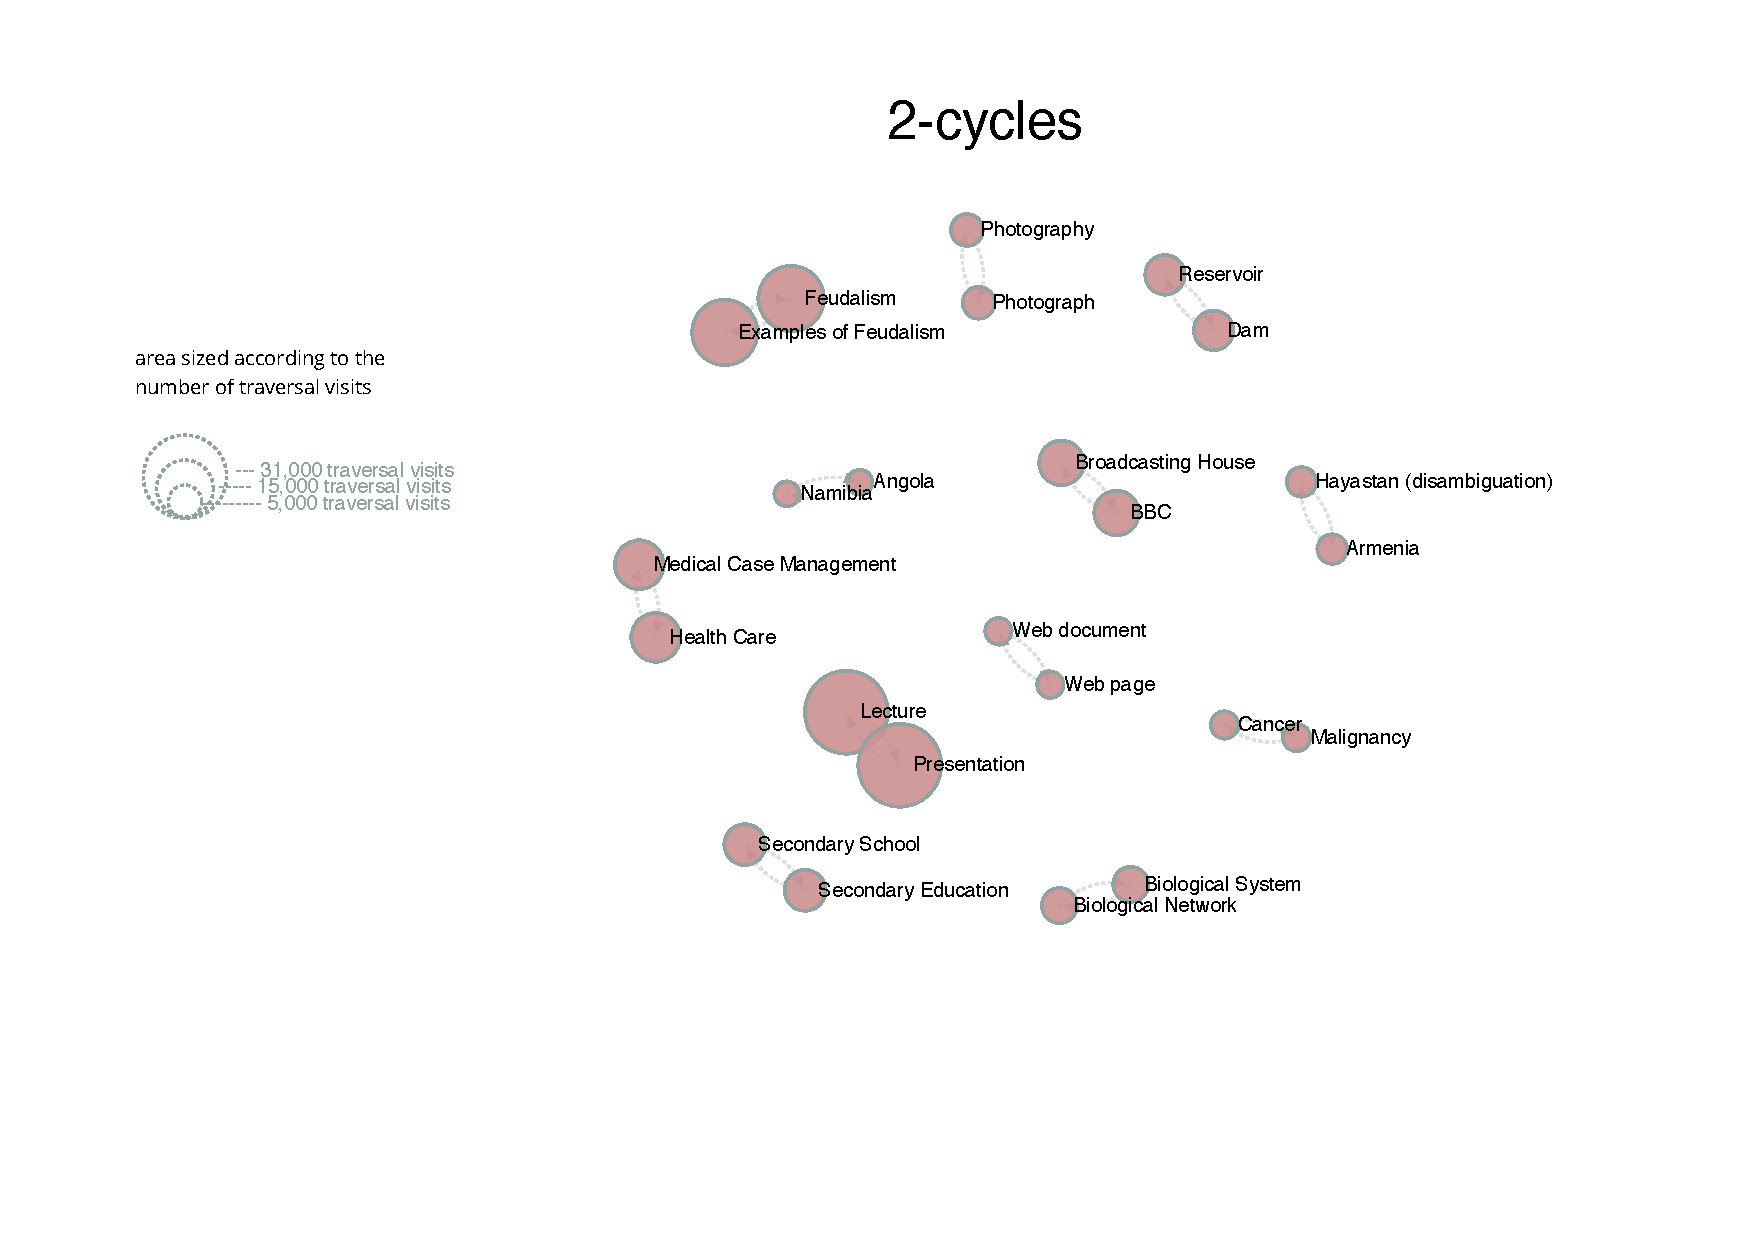
\includegraphics[width=\textwidth]{graphics/2_cycles.pdf}
  \caption{
    \textbf{Highest ranking 2-cycles.}
    We identify pairs of articles whose First Links point to one another, forming
    a 2-cycle. We then rank each pair of articles by the total number of 
    traversal visits to gauge the most referenced groups of two articles linked
    to each other. The area of the circles in the figure indicates the number of traversal visits. We find 2-cycles often capture synonyms or articles representing nearly the 
    same concepts as opposed to distinct ideas.
  }
  \label{fig:2-cycles}
\end{figure*}

Outside of the highest ranking 2-cycles, the typical 2-cycle signals a connection between distinct, yet very closely related ideas. 
We also observe link patterns such as inventor to product ("Voere" to "VEC-91"), event to organizer ("Poetry Bus Tour" to "Weave Books"), and book to author ("Anatomy of Britain" to "Anthony Sampson").

Similarly, 3-cycles capture a synonymous or close relation among 3 articles: "Tree of life (Biology)", "Tree of life (disambiguation)", 
and "Tree of life"; "Cinema of India", "Indian Cinema", and "Telugu Cinema"
(see figure~\ref{fig:3-cycles}).
Once we extend our cycle size beyond a length of 6 however, 
"Philosophy" along with the remaining list of high ranking articles by traversal visits dominate.
The longest cycle in the network spans 365 articles of Eastern Orthodox Liturgics for each calendar day.
Other lengthy cycles span 60-75 articles including collections of articles on national histories such as "Japanese Eras" 
or judicial bodies such as the "Legislative Assembly of Ontario".

\begin{figure*}[tp!]
  \centering	
  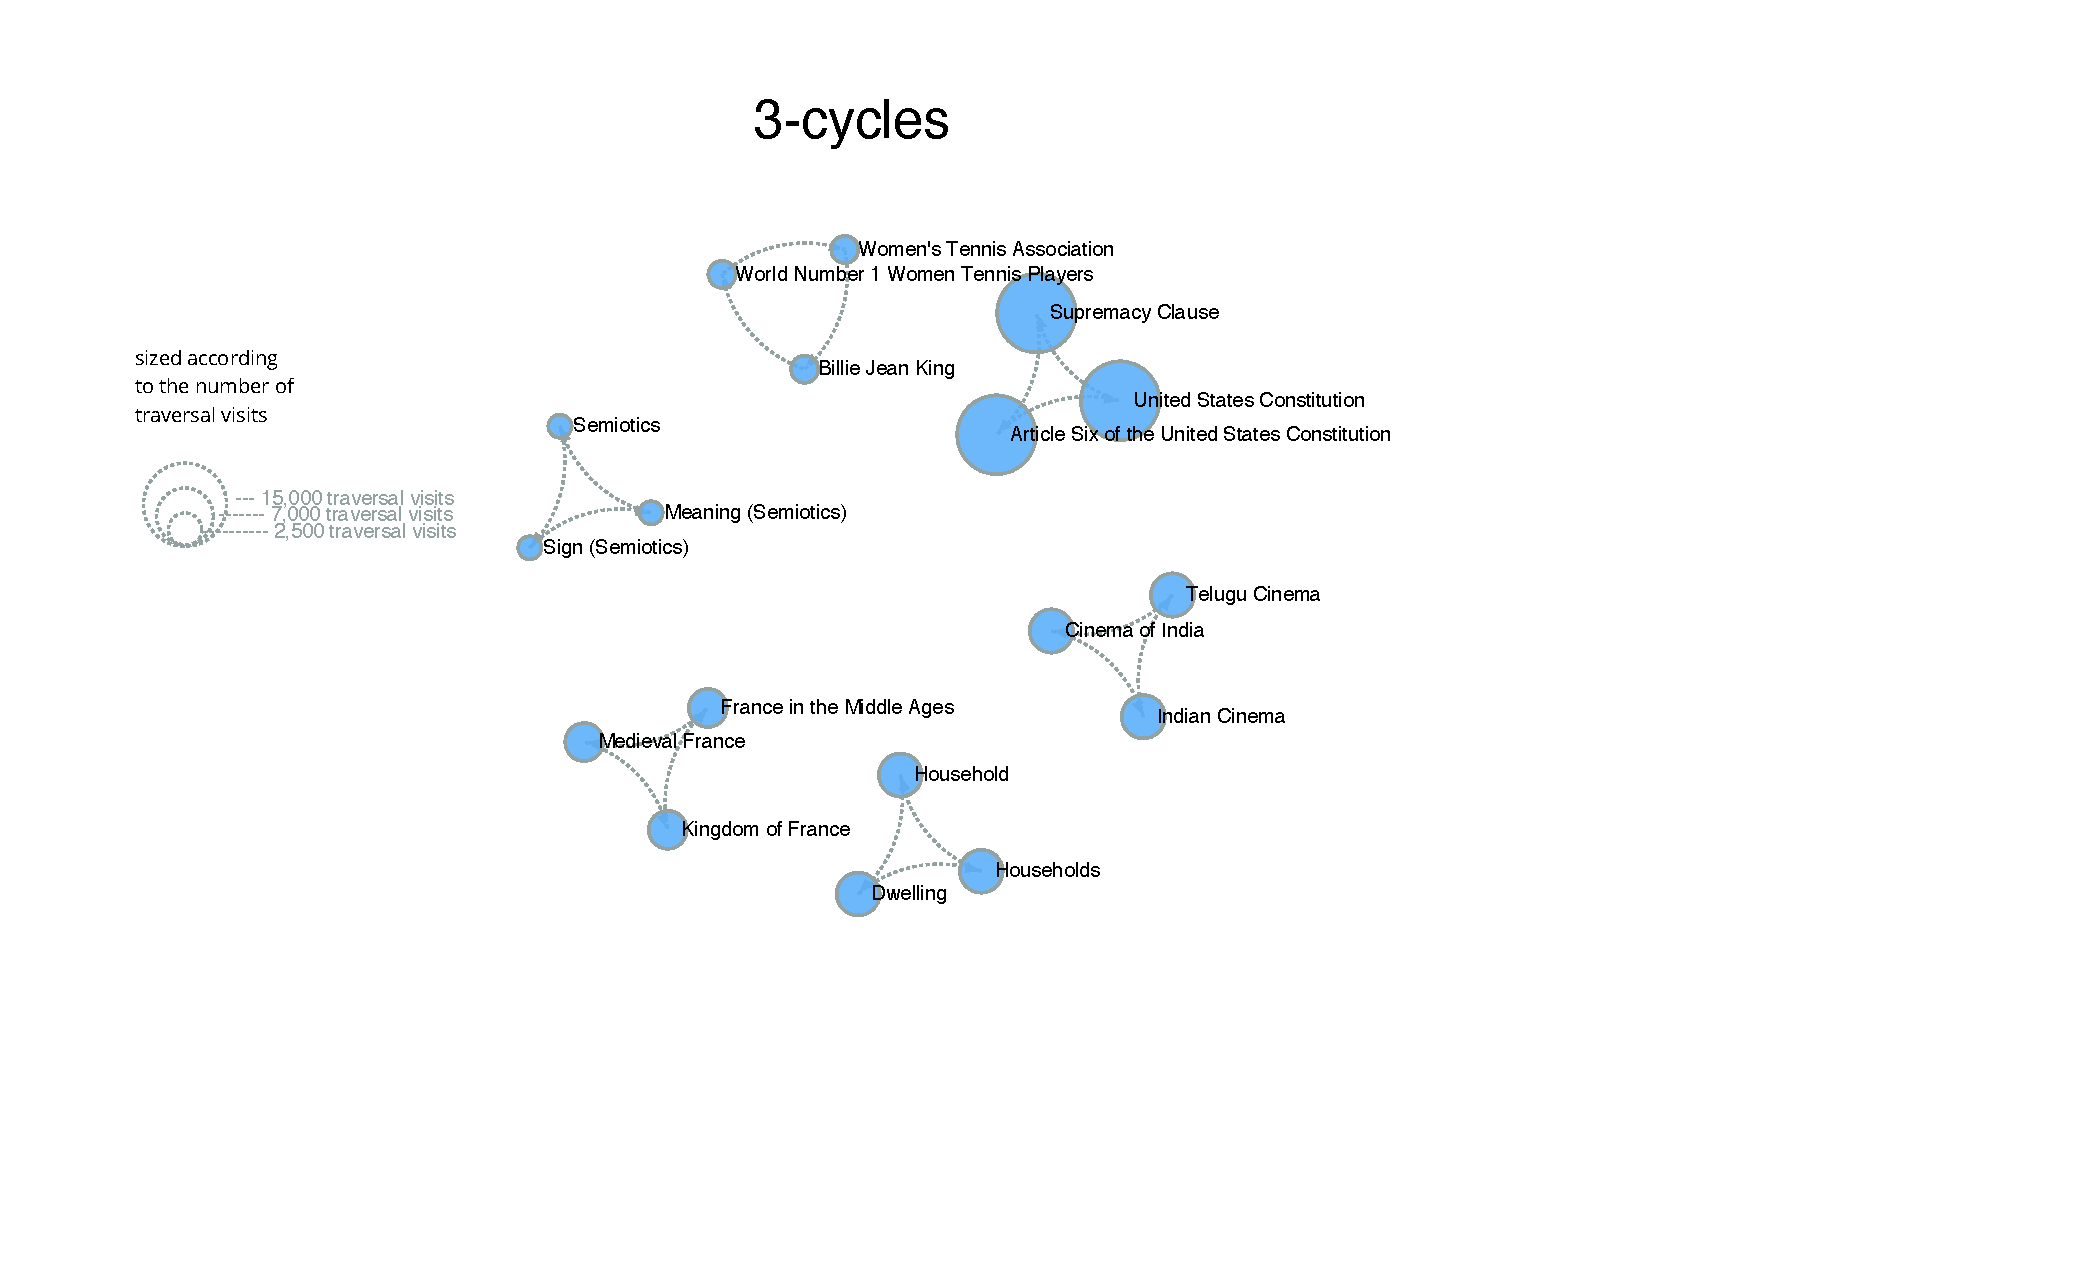
\includegraphics[width=\textwidth]{graphics/3_cycles.pdf}
  \caption{
    \textbf{Highest ranking 3-cycles.}
    We identify groups of three articles whose links form a 3-cycle with the 
    last article in the group linking back to the first article.
    We rank each 3-cycle by the total number of traversal visits to gauge
    the most referenced group of three linked articles. 
    The area of the circles in the figure indicates the number of traversal visits. 
  }
  \label{fig:3-cycles}
\end{figure*}






\subsection{Basins}

We can group articles lying on the same path to identify {\it basins}: 
a group of path-connected articles.
Since cycles identify only groups of articles with a closed set of links, 
we additionally measure and rank basins to capture groups of closely related
articles branching outside of a cycle into the rest of the FLN.
We rank basins by the total number of traversal visits for each article in the path. 
Akin to river networks, these basins are areas of accumulation with a path 
flowing outwards to the rest of the FLN.

The highest ranking basins by the number of traversal visits are groups of articles
around "Philosophy." 
Since the accumulation of First Links to "Philosophy" is so high, 
the paths leading to "Philosophy" carry many references.
The highest ranking paths include branches of philosophy flowing through 
"Awareness,"Existence," and "Consciousness" to "Philosophy." Other paths
include concepts around "Mathematics," scientific "Experiments," 
"Biology," and "Fact."
These paths link many specific articles to "Philosophy," each funneled through a particular domain.

Excluding basins around "Philosophy," we find other basins around 
foundational ideas such as "Community," "Landmass," "Federal Government," 
"Presentation," and "Belief System." 
The basins around each of these foundational notions are 
various paths containing related articles. For example around 
"Community" we find basins
flowing from "United States" to "Federal Republic" to "Political Union" to "State" culminating at "Community"; we also find basins flowing from 
"Public Policy" to "Executive (government)" to "Government" to State" and then 
to "Community"; we also find paths flowing through a similar chain beginning
with "Democracy," another beginning with "Constitution," another at 
"Dictatorship," and so on. The ideas build from specific means of organizing
a community (or society) and then build up to "Community." 
Other basins around landmass for example begin at specific geographical regions
such as "Eastern Europe" building up to "Continent" and finally "Landmass."
Each basin groups First Link references through various 
natural paths linking general themes to the foundational concept.

Which specific articles direct the path towards a particular concepts? 
Next we study the FLN using traversal funnels to understand the influence
a particular article exerts in directing the flow of First Link references.



\subsection{Traversal Funnels}

To analyze the influence an article exerts in shaping the 
structure of the FLN, we compute the number of traversal funnels for each.
Articles directing more paths exert a greater influence over the structure
of the FLN by increasing the accumulation of First Links
on a particular path. By measuring traversal funnels, we distinguish between an article that simply happened to fall within a cycle from an article funneling 
many First Links.

Ranking articles by the number of traversal funnels we find 
"Philosophy" as by far the highest-ranking article with 
$7.37$ million paths
(see figure~\ref{fig:Funnels}).
\begin{figure*}[tp!]
  \centering	
  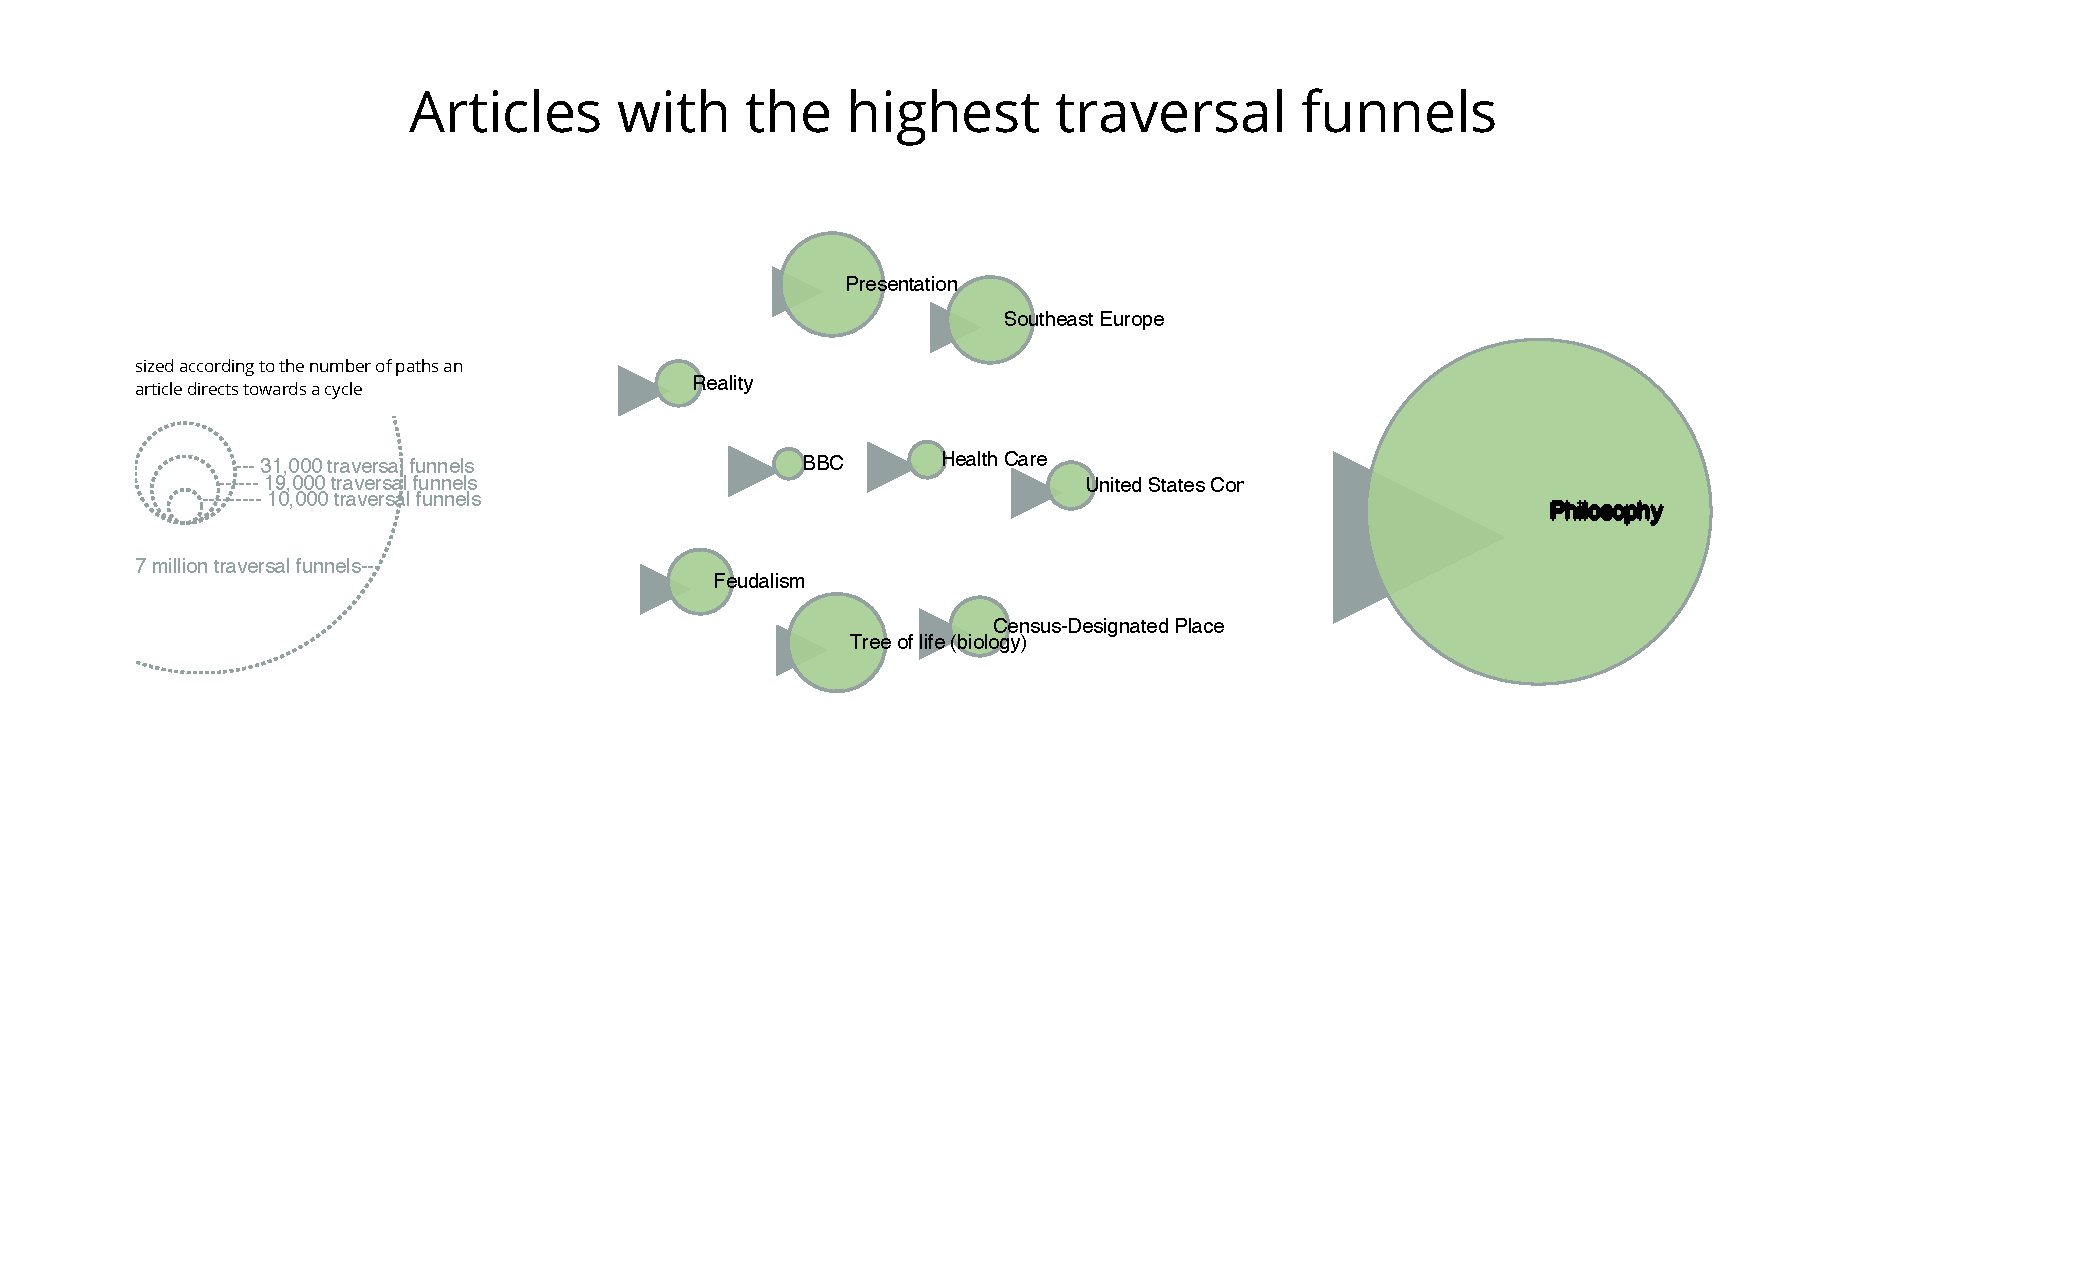
\includegraphics[width=\textwidth]{graphics/funnels.pdf}
  \caption{
    \textbf{Funnels.}
    We represent the highest-ranking articles by the number of traversal 
    funnels to gauge the influence each article exerts in shaping the 
    structure of the FLN. We find "Philosophy" exerts an overwhelming proportion
    of the influence, with other abstract notions and topical concepts ranking
    next.
  }
  \label{fig:Funnels}
\end{figure*}
Of any article, the number of traversal funnels Philosophy holds exceeds 
all others by more than two orders of magnitude.
The "Philosophy" cycle which contains "Existence," "Awareness," "Reality," 
and similar articles accumulates the overwhelming proportion of its 
references through "Philosophy": $7.37$ million of the $7.4$ million references
are funneled through "Philosophy."
Second on the list of highest-ranking articles by traversal funnels is 
"Presentation" with only $30$ thousand paths. Similarly abstract 
ideas also rank highly such as "Tree of life" (30 thousand), 
"Reality" (13 thousand), and "Jurisdiction" (3 thousand).

Many high-ranking articles are remarkably topical, culturally and politically important ideas.  For example, "Health Care", a recently high-contested legislative topic appears high on the list---Google trends indicates an uncharacteristic spike in search frequency between August-2009 and February-2010.
Other high ranking articles include key historical events such as the "Cold War" or critical scarce resource with recent 
media discussion such as "Fossil Fuel". 
The highest-ranking list even includes "Hip Hop," "Cancer," and "Web Page."
This coincidence of recent relevance and traversal funnel rank suggests the First Link Network measurably represents
meaningful relationships not only among ideas, but also to English-speaking society. 
\begin{figure}[tp!]
  \centering	
  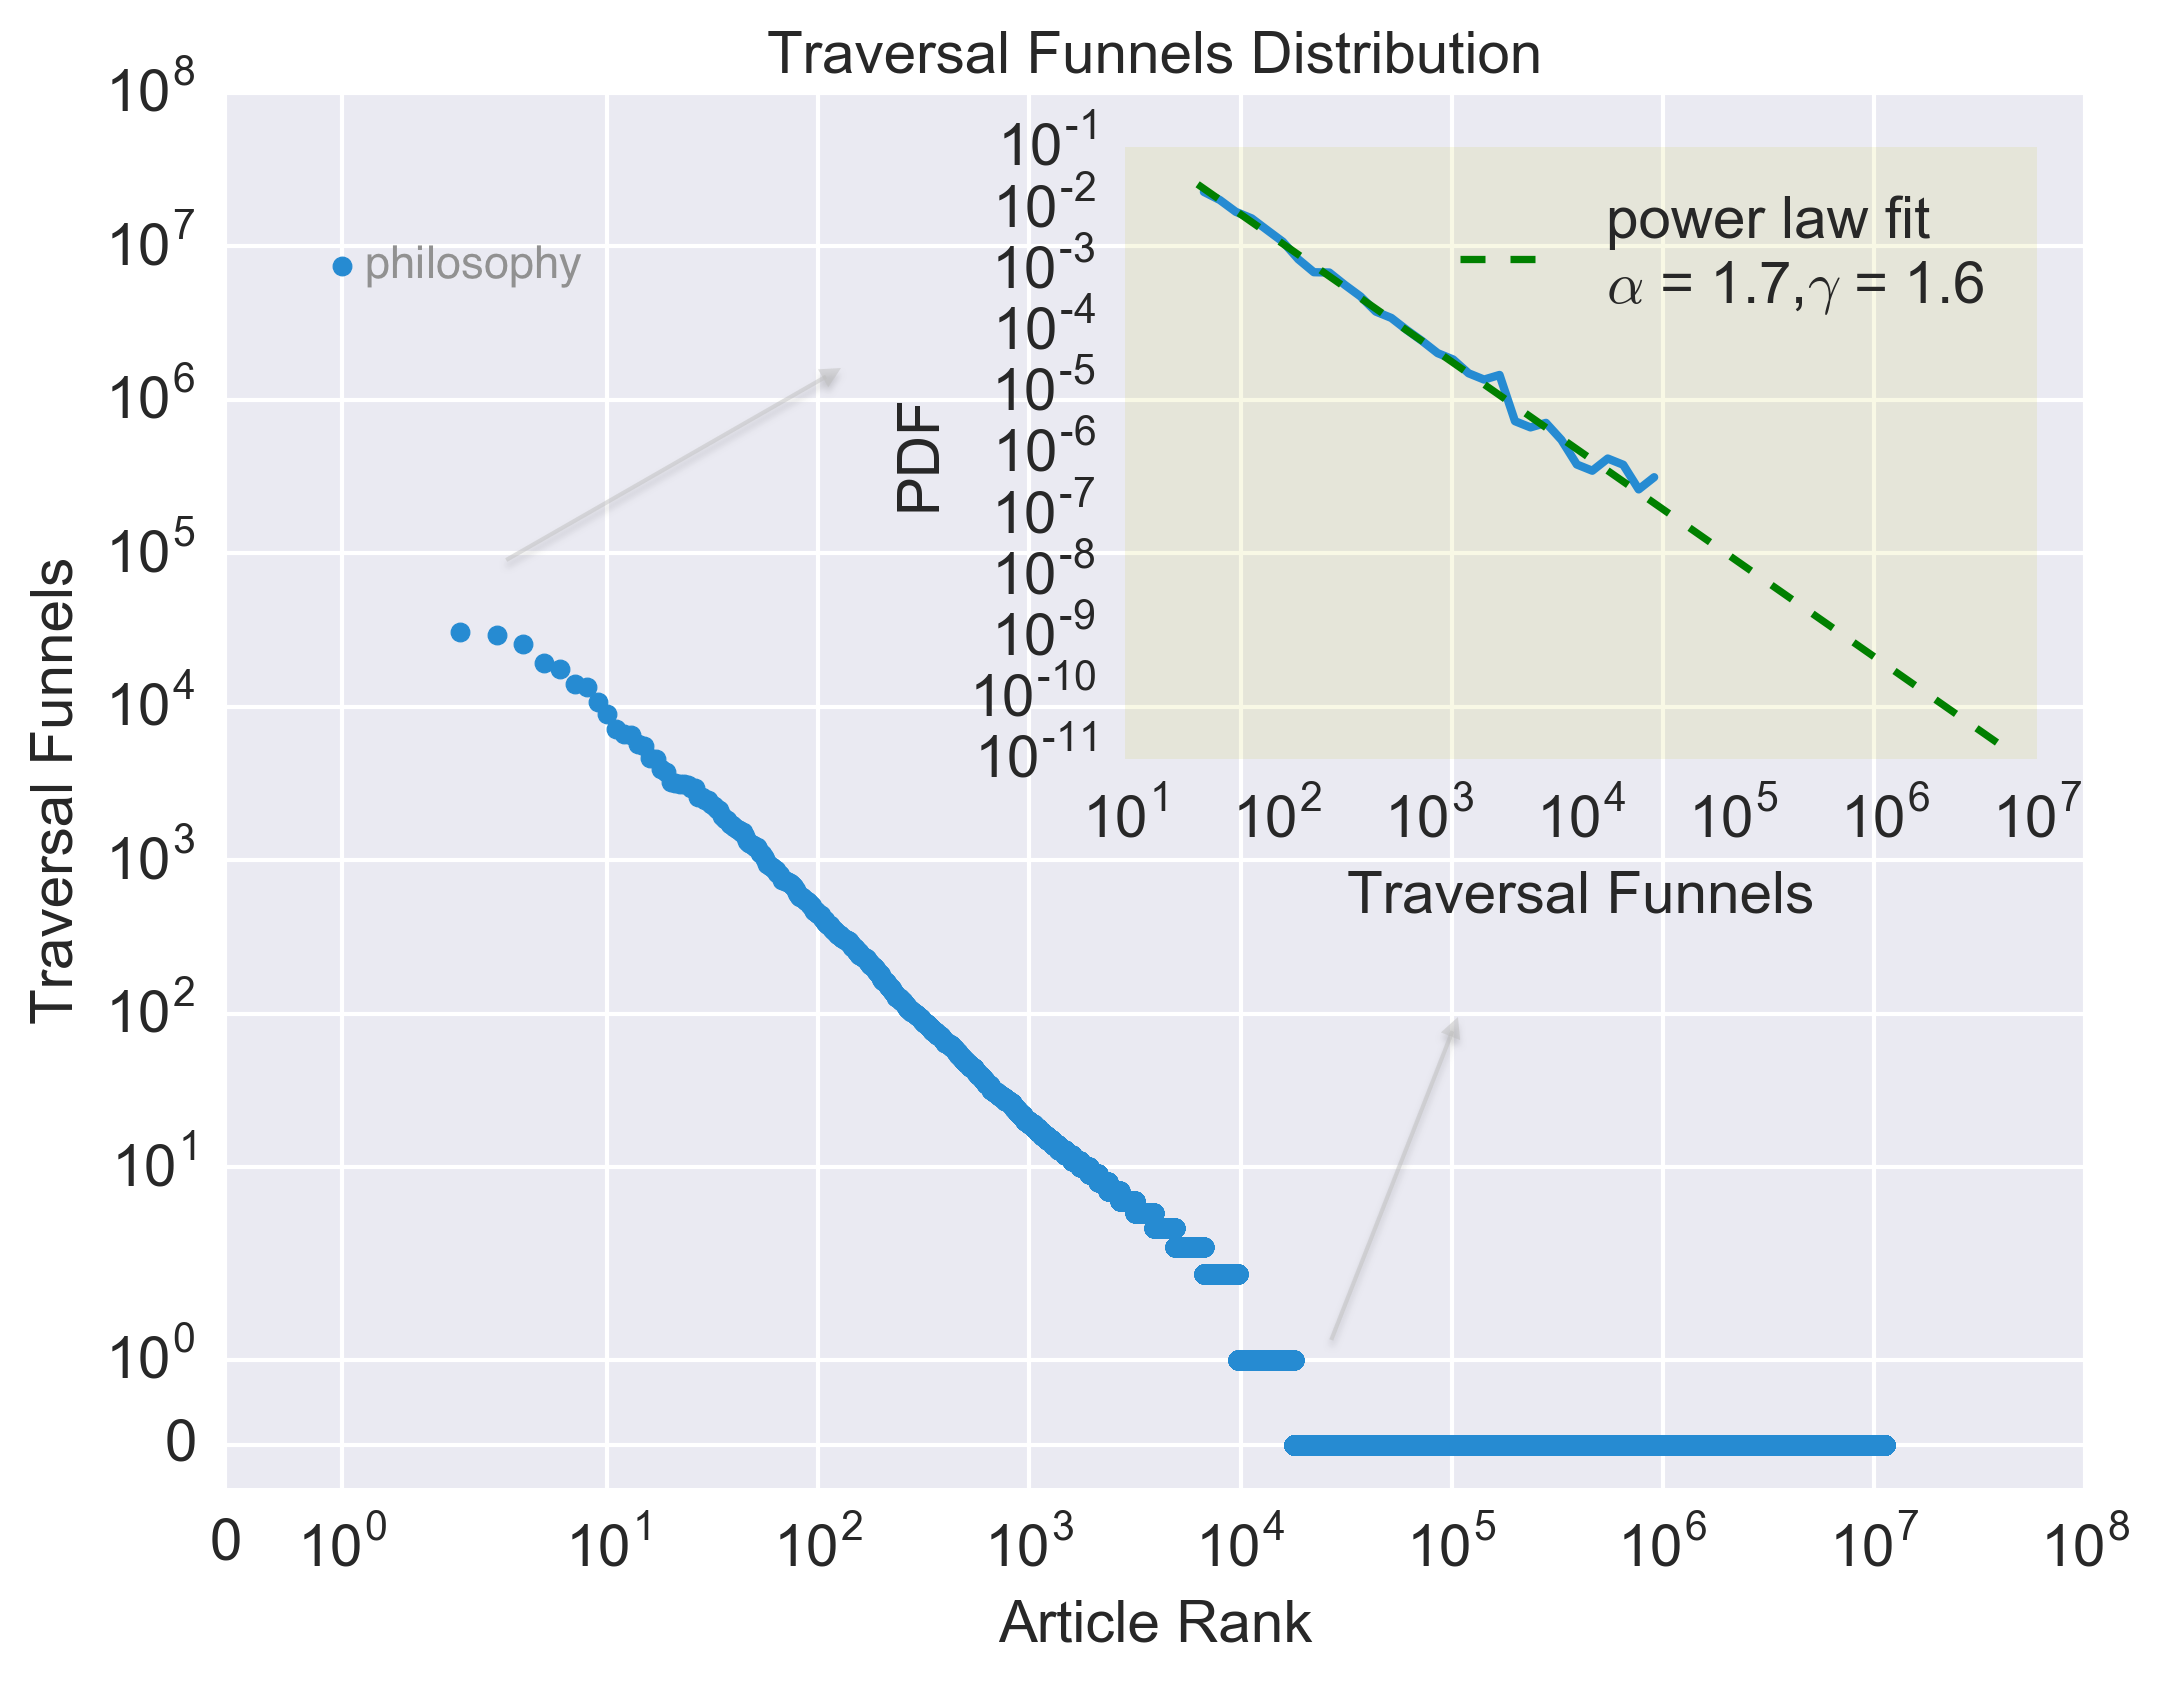
\includegraphics[width=\columnwidth]{graphics/funnels_distribution.png}
  \caption{
    \textbf{Distribution of Traversal Funnels.}
  We fit the distribution with a linear log-log model by considering the log (base 10) transformed rank of each article against log (base 10) transformed the number of traversal funnels. 
  We find two regimes with the top regime (log(rank) < 4) 
  well-explained by a linear fit, yielding an r-value of $-0.99$ and a 
  power-law exponent of $-1.08$. The top regime 
  explains the distribution of traversal funnels for the $17, 821$ 
  articles with at least one traversal funnel. The bottom 
  horizontal regime corresponds to the more than $99\%$ of articles
  which hold zero traversal funnels.
  }
  \label{fig:Funnels Distribution}
\end{figure}

As a distribution, we find few articles influence the structure of the 
FLN. Only $17, 821$ articles have one or more traversal funnels, leaving
an more than $99\%$ with none---most articles are recipients of 
the references flowing through the articles with at least one traversal funnel.
When fit to a log-log linear model we find the $99\%$ of articles with zero
traversal funnels form one regime (with log(rank) less than 4).
The top regime, corresponding to the $17, 821$ articles with at least one 
traversal funnel strongly fits a linear model with an r-value of $-0.99$. 
The resulting power-law exponent is $-1.08$. Even within the few articles
influencing the structure of the FLN, only a handful of these exert most of the 
control. 

The flow of ideas in the FLN is overwhelmingly influenced by "Philosophy,"
with a small proportion guided by "Presentation," "Tree of life (biology)," "Southeastern Europe," 
"Feudalism," "Census-Designated Place," "United States Constitution," "Reality," and "Health Care."



\subsection{Article Popularity}

Wikipedia released an API to measure article popularity by page views
starting November 2015. Page views add another dimension to our
findings by revealing 
how users view the information on Wikipedia. 
We measure popularity as the total number 
of page views in the English edition of Wikipedia in the month of 
October 2015---the earliest full month for which the data is available. 
We find the highest ranking 1000 articles (by traversal visits) have an average of
$70$ thousand page views in October with high variation: the standard deviation 
is $1.1$ million page views. 
The number of page views has a skewed distribution with $75\%$ of articles
reaching fewer than $73$ thousand page views in October.
The article for "United States" has the most page 
views of the highest ranking $1000$ articles by traversal visits with 
$1.4$ million views in October. The next most popular articles are 
"India," "World War II," and the "United Kingdom" each with $0.7-1.03$ million page views. 


The "Philosophy" article despite outranking every article by traversal visits,
has only $240$ thousand page views in October compared to the $1.4$ million
page views for "United States".
While "Philosophy" is not itself the most popular article, "Philosophy" serves as 
an accumulation point for ideas. Wikipedia users do not login specifically
to read about "Philosophy," but the authors relate ideas to "Philosophy" 
by ultimately anchoring the flow of First Links to "Philosophy."

\begin{figure}[tp!]
  \centering	
  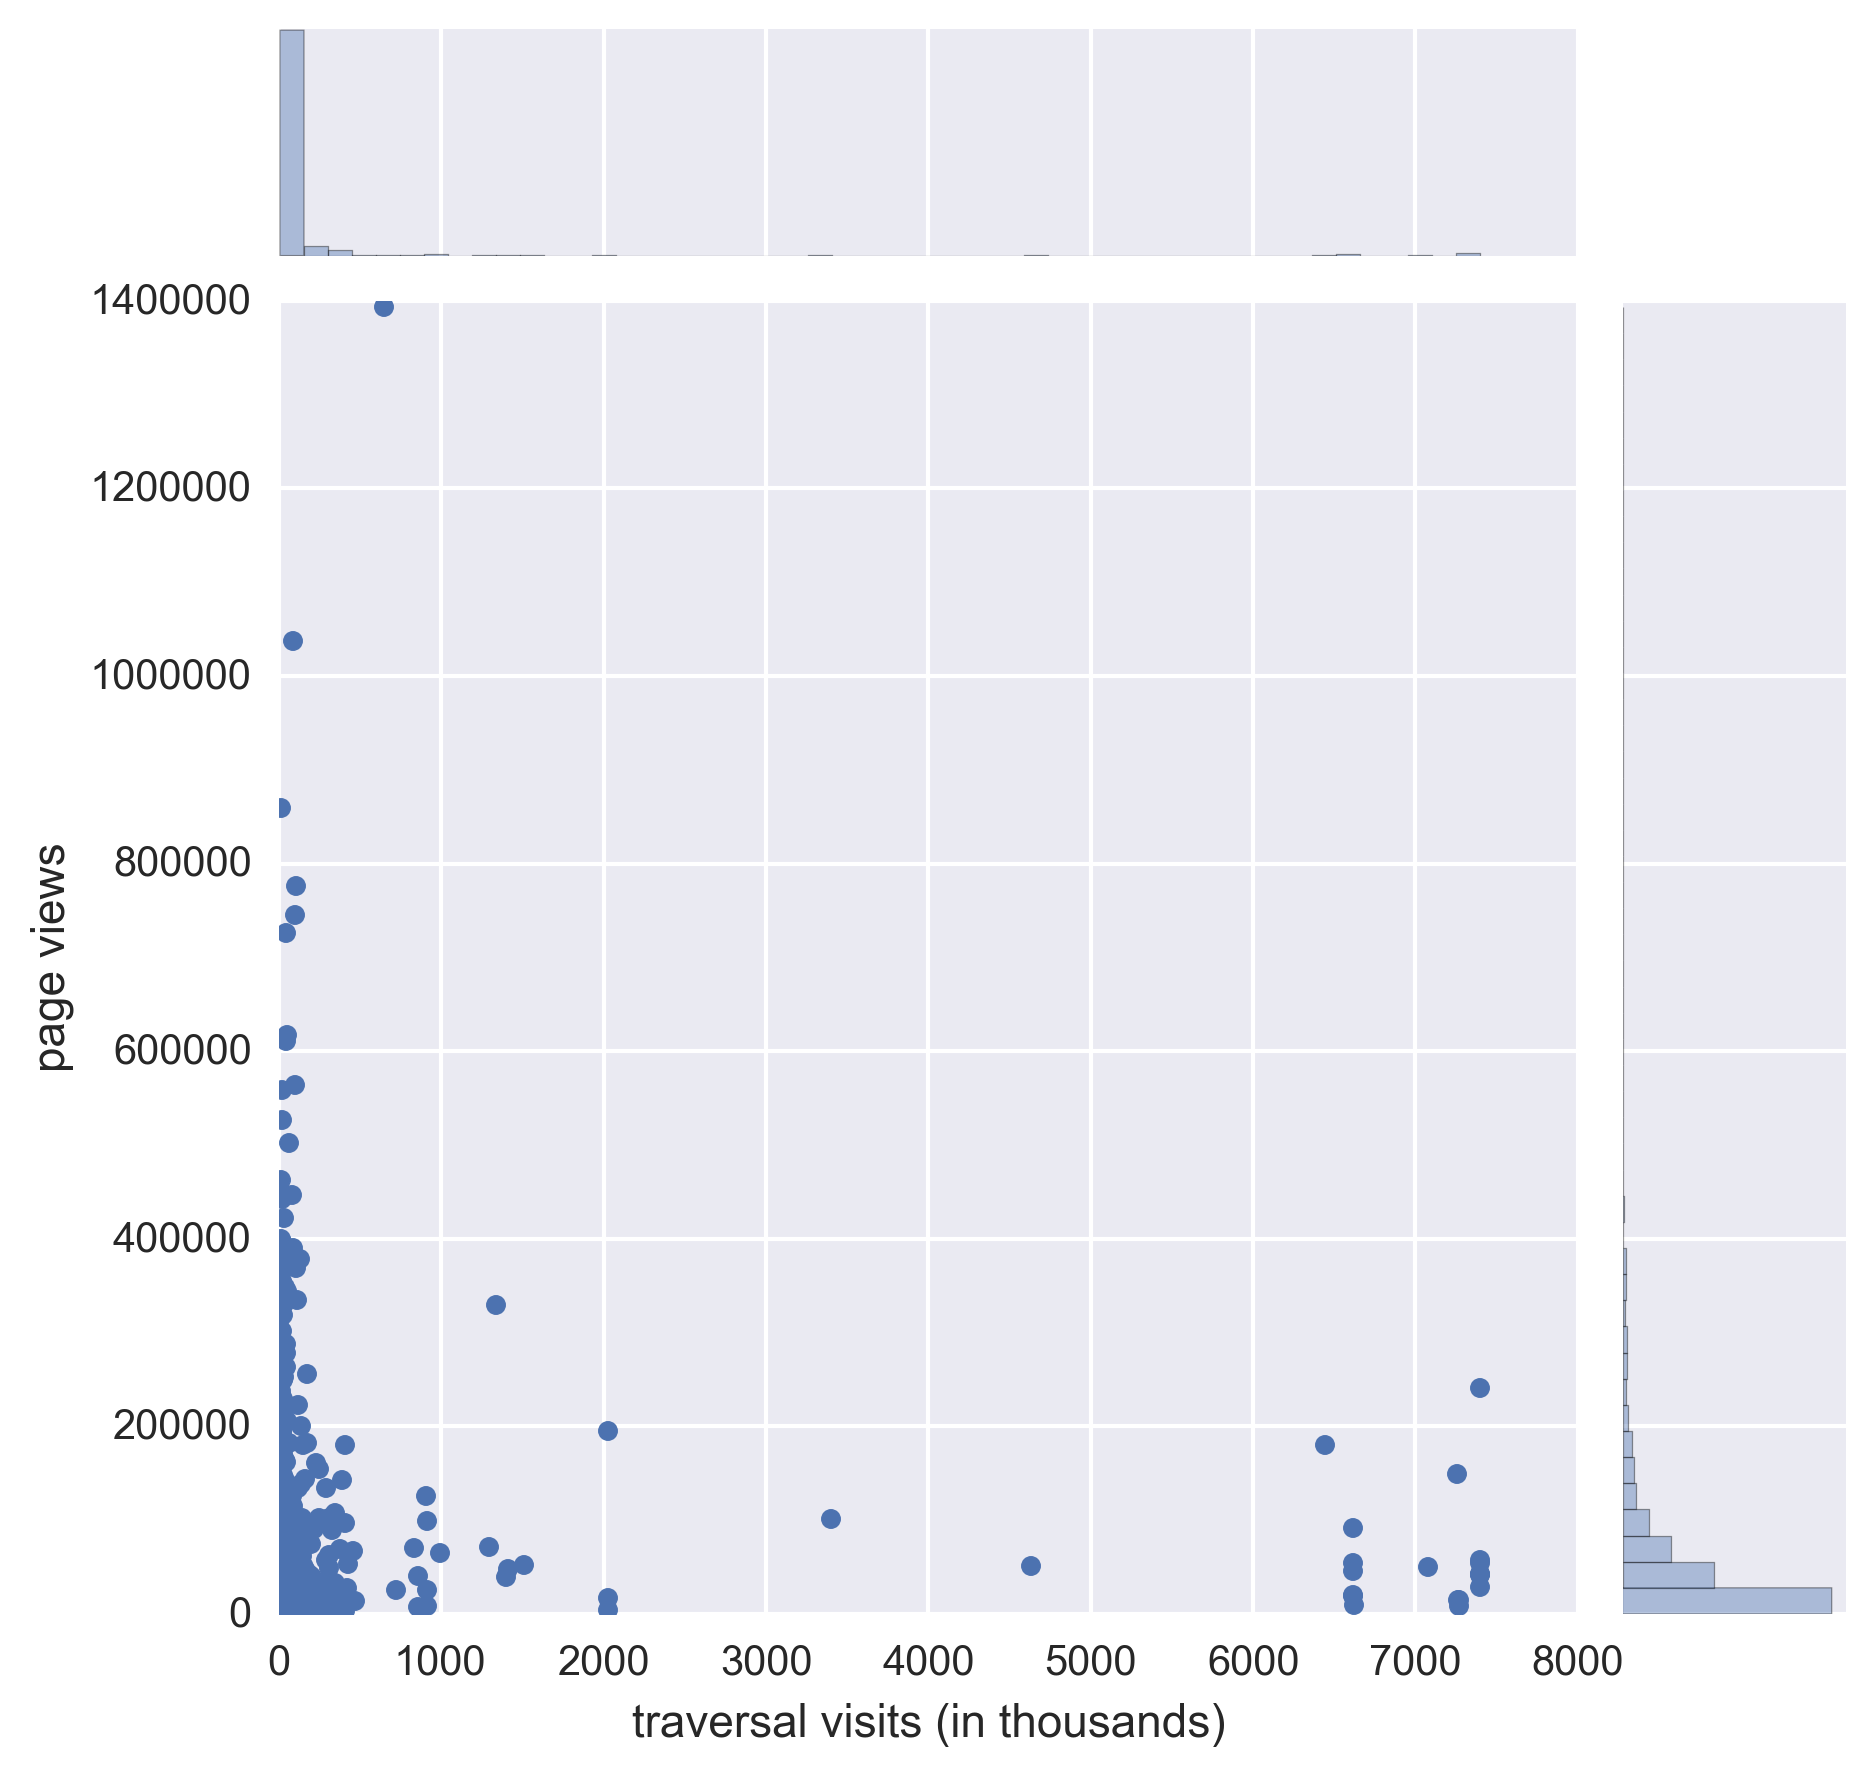
\includegraphics[width=\columnwidth]{graphics/views_visits.png}
  \caption{
    \textbf{Article Popularity (by page views) compared to Traversal Visits 
    for Highest ranking 1000 articles.}
    We use the total number of page views provided by Wikipedia for the month
    of October 2015 to compare each article's popularity to traversal visits.
    While the most popular articles do not necessarily correspond to the articles
    with the highest number of traversal visits, the variation in popularity appears to decrease as the number of traversal visits increases.
  }
  \label{fig:Views and Visits}

\end{figure}



We also analyze article popularity for the highest ranking 1000 articles by 
traversal funnels. In October, the average page views per article is 
$22$ thousand with a standard deviation of $95$ thousand views. The distribution
is skewed with $75\%$ of articles reaching fewer than $20$ thousand page views. 
"Halloween" is the most popular article with $2.8$ million views in October,
likely a result of Halloween falling in the month of October. 
Other popular articles include "Scientology" ($463$ thousand views), "Clint Eastwood" 
($341$ thousand views),
and the "Cold War" ($298$ thousand views) although each has significantly fewer views compared to the views for "Halloween."
Other standout popular October articles include "24-hour" and "12-hour" clocks likely due
to Daylight savings in October and "Marriage" likely due to the drop in the number of
weddings in the months following October
\cite{weddings}.
"Philosophy" which ranks seventh among the most popular of the highest ranking articles by traversal funnels, appears no where in the top 20
by traversal visits. "Philosophy" is a relatively popular article 
among articles influencing the shape of the network, but less popular among 
highly-ranked articles by accumulation.


\begin{figure}[tp!]
  \centering	
  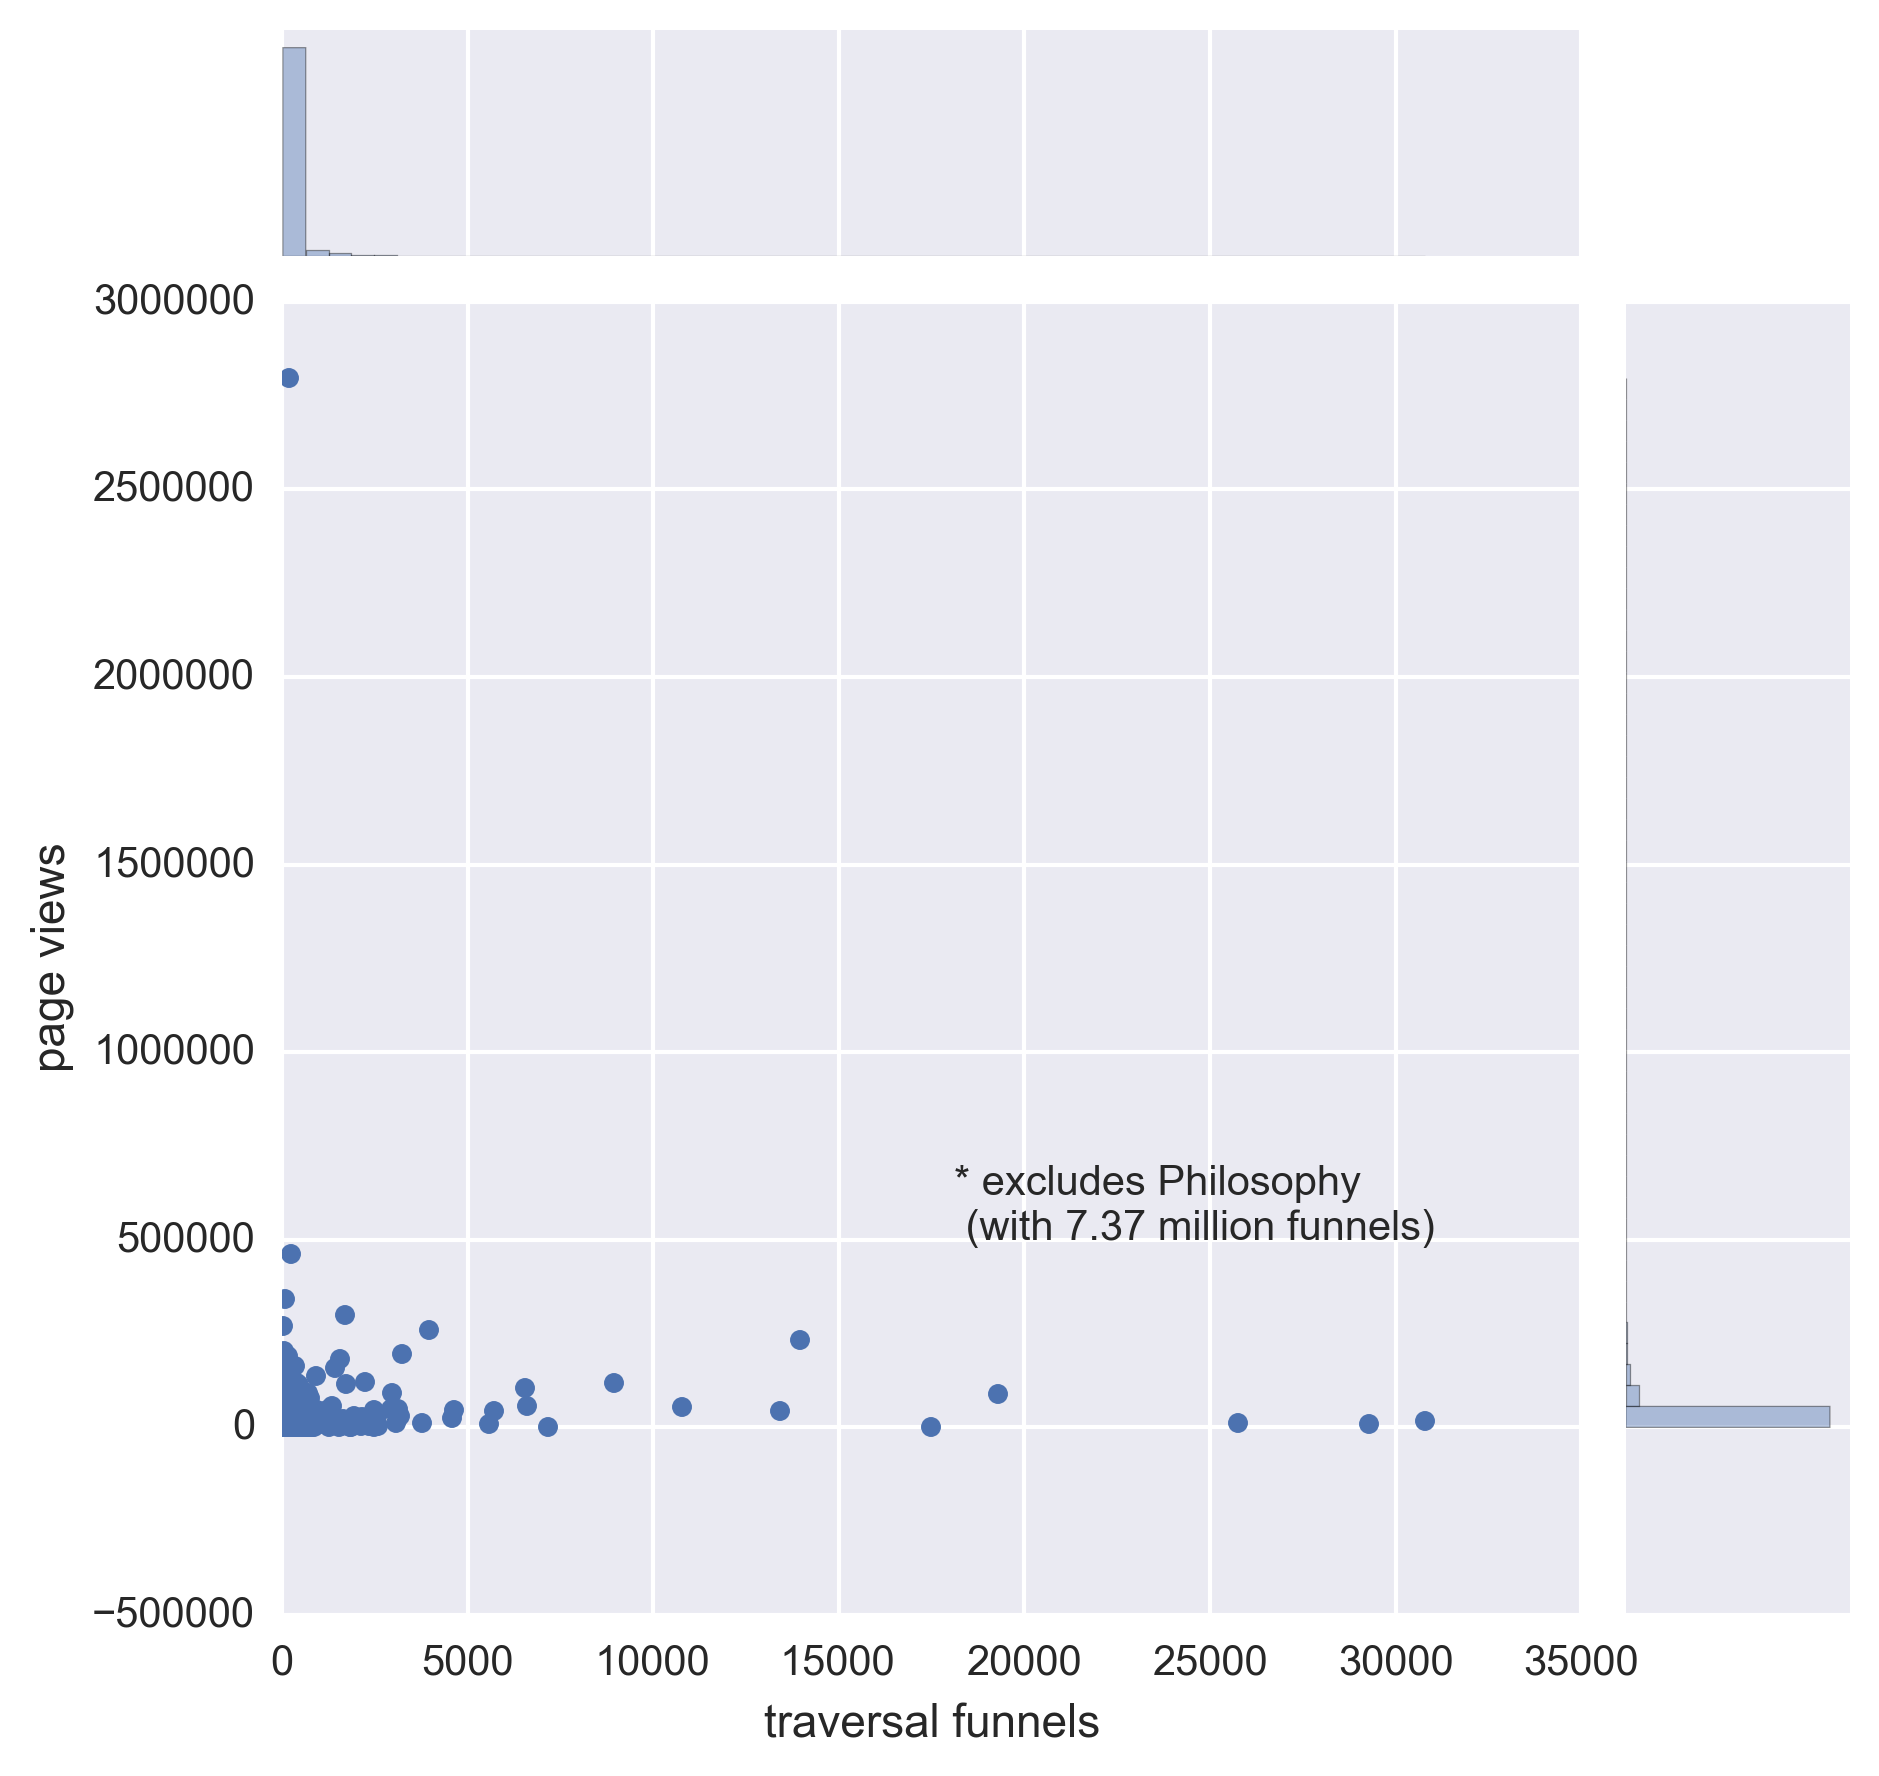
\includegraphics[width=\columnwidth]{graphics/funnels_visits.png}
  \caption{
    \textbf{Article Popularity (by page views) compared to Traversal Funnels
    for Highest ranking 1000 articles.}
  }
    We use the total number of page views provided by Wikipedia for the month
    of October 2015 to compare each article's popularity to traversal funnels.
    In the top left is "Halloween" with a significantly greater 
    number of page views in the month of October.
  \label{fig:Views and Funnels}
\end{figure}



%========================Conclusion====================================

\section{Reflections}

The findings here should only be considered within the limitations of their context.
We examined only the English version of Wikipedia at a particular moment in time.
Furthermore, we only studied the First Link in the main body  of each article
as a means to related one article to another. Finally, Wikipedia, while the largest 
collection of human knowledge, is rife with the biases of the many contributing editors
\cite{bias}
. Nevertheless, the findings do reveal
generalizable relationships, point to foundational notions, and uncover many curiosities.


Among the curiosities is the multiple appearance of scale-free distributions within the network. 
The three metrics we developed: path length, traversal visits, and traversal funnels are all marked 
by scale-free distributions. Few articles have most traversal visits, few paths have an exceptionally long path length, and even fewer
articles are responsible for funneling most paths. When measured against the traversal funnels, 
"Philosophy" emerges as an exceptional article by orders of magnitude. 
Nevertheless, many other foundational ideas emerged naturally within the First Link Network. 
Basins around "Community", "State", and "Science" reveal a foundational structure within the network. 
More curious is the emergence of recently prominent political and economics topics such as "Fossil Fuel" and "Health Care" 
within the highest ranking funnels. 
Wikipedia seems to reflect not only timeless foundations, but also the topical (at least within English speaking society).

Future work could examine other language versions of Wikipedia for potentially telling cultural or regional differences as well as expand the network to more than the First Link.
These findings also form the basis for the creation of a taxonomy where 
every idea, event, or object sits within a hierarchy of connected notions.
The taxonomy would extend a traditional word thesaurus beyond mere synonyms to a related hierarchy of concepts.
Applications could range from an enhanced thesaurus of ideas to psychological insights into how humans form associations.
Specifically, an ever-evolving reference of related hierarchical concepts can be applied to search engine algorithms 
or natural language processing.


\acknowledgments
Thank you to my friend RJ for pointing out the Reddit post 
\cite{reddit}
describing how the majority of links lead to "Philosophy," inspiring this research.


\newpage

\section{Appendix}

\subsection{Constructing The First Link Network}

To map Wikipedia's First Link Network, we use the freely-available XML dump of the English edition of Wikipedia. 
Rather than rely on a sample of articles from which to generalize, we opted to process the entirety of Wikipedia, 
eliminating any statistical error due to sampling.
We analyze the snapshot provided on November 2014, representing the state of Wikipedia at the time.
The November raw dump consists of 11 million articles: 4.7 million unique articles along with redirects
and disambiguations.
Knowing Wikipedia is an ever-evolving project with 10 edits every second and 750 new articles per day on average
\cite{wiki_edits},
our aim is to characterize the dynamics of the First Link Network, not record a particular link between one
article and another.

Wikipedia renders and stores articles in MediaWiki markup, a markup language with syntax and keywords to format and mark elements in a page. Along with special syntax for links, MediaWiki markup includes templates for audio files, images, and side-bar
information.
While a human could accurately identify the First Link, to map the entire First Link Network of 11 million articles, we needed to programmatically untangled the body text from side-bar, header box, and invalid link elements.

While some libraries exist for MediaWiki Markup,
Approaches using existing libraries led to several bugs 
including trouble with nested links, nested parenthesis, unclosed tags, escape characters 
as well as compatibility with other libraries used to parse the XML.
Consequently,  we developed an algorithm for parsing the First Link in the XML version of each article.
Our parsing algorithm aimed to: 
1) accurately identify the First Link among other page elements, and 
2) efficiently do so---that is without needing for several passes through the data.
To process an article in a single pass, we developed a hierarchical system of flags:

\begin{figure}[tp!]
  \centering	
  \includegraphics[width=\columnwidth]{graphics/flags.pdf}  
  \caption{
    \textbf{Parsing Algorithm of Wikipedia's XML dump.}
     The highest flag in the hierarchy indicates a Wikimedia template used to mark an element in the side bar, display an image, link to an external file, or another Wikimedia project outside of Wikipeida. Next, to catch any remaining elements outside the main body we have a second flag for <ref>, <div> elements. Finally, we identify parenthesis to ensure we do not capture a link to a pronunciation key.
  }
  \label{fig:parsing algorithm}
\end{figure}

The algorithm loops in three-character chunks to account for potentially nested elements, 
shifting by one character steps through the article markup.
If any markup triggers for a flag are detected, a flag is raised. 
Once a flag is raised, we stop processing and proceed to the next character
until the flag's closing markup.
A First Link is identified only if Flags 1, 2, and 3 are all off.
In this case, the entire link is retrieved. 
We then confirm the link is valid by filtering for MediaWiki keywords indicating external page or other projects
as well as common file extensions for 
images, audio files, and the like 
\cite{media_wiki_templates}.
The First Link of an article is then the earliest valid link with unraised flags.

To process the entirety of Wikipedia, we distributed the parsing and processing of the XML dump
across 112 cores of the UVM supercomputer cluster
\cite{vacc}
We then joined the results to form a hash table containing every Wikipedia article and its corresponding
First Link. The resulting network map is the basis of our analysis.





\begin{thebibliography}{1}

      \bibitem{editors} Iba, Takashi, et al. "Analyzing the creative editing behavior of Wikipedia editors: Through dynamic social network analysis." Procedia-Social and Behavioral Sciences 2.4 (2010): 6441-6456.

      \bibitem{accuracy1} Holman Rector, Lucy. "Comparison of Wikipedia and other encyclopedias for accuracy, breadth, and depth in historical articles." Reference services review 36.1 (2008): 7-22.

      \bibitem{accuracy2} Giles, Jim. "Internet encyclopaedias go head to head." Nature 438.7070 (2005): 900-901.

       \bibitem{coverage} Halavais, Alexander, and Derek Lackaff. "An analysis of topical coverage of Wikipedia." Journal of Computer‐Mediated Communication 13.2 (2008): 429-440.

        \bibitem{bias_women} Hill, Benjamin Mako, and Aaron Shaw. "The Wikipedia gender gap revisited: characterizing survey response bias with propensity score estimation." PloS one 8.6 (2013): e65782.

      \bibitem{missing_entries} Williams, Jake Ryland, Clark, Eric M., Bagrow, James P., Danforth, Christopher M. \& Dodds, Peter Sheridan (2015). Identifying missing dictionary entries with frequency-conserving context models. Phys. Rev. E, 92, 042808.

      \bibitem{clustering} Banerjee, Somnath, Krishnan Ramanathan, and Ajay Gupta. "Clustering short texts using wikipedia." Proceedings of the 30th annual international ACM SIGIR conference on Research and development in information retrieval. ACM, 2007.

      \bibitem{semantic_relatedness} Gabrilovich, Evgeniy, and Shaul Markovitch. "Computing Semantic Relatedness Using Wikipedia-based Explicit Semantic Analysis." IJCAI. Vol. 7. 2007.

      \bibitem{disambiguating} Cucerzan, Silviu. "Large-Scale Named Entity Disambiguation Based on Wikipedia Data." EMNLP-CoNLL. Vol. 7. 2007.

      \bibitem{drugs} Clauson, Kevin A., et al. "Scope, completeness, and accuracy of drug information in Wikipedia." Annals of Pharmacotherapy 42.12 (2008): 1814-1821.

      \bibitem{stats} Wikipedia contributors. "Wikipedia:Statistics." Wikipedia, The Free Encyclopedia. Wikipedia, The Free Encyclopedia, 9 Nov. 2015. Web. 13 Nov. 2015.

      \bibitem{pagerank} Page, Lawrence, et al. "The PageRank citation ranking: bringing order to the Web." (1999).

      \bibitem{classifier} Chakrabarti, Soumen, Mukul Joshi, and Vivek Tawde. "Enhanced topic distillation using text, markup tags, and hyperlinks." Proceedings of the 24th annual international ACM SIGIR conference on Research and development in information retrieval. ACM, 2001.

      \bibitem{relevance} Kamps, Jaap, and Marijn Koolen. "Is Wikipedia link structure different?." Proceedings of the second ACM international conference on Web search and data mining. ACM, 2009.
          
      \bibitem{wiki_train} Wikipedia contributors. "Train." Wikipedia, The Free Encyclopedia. Wikipedia, The Free Encyclopedia, 
          \url{https://en.wikipedia.org/wiki/Train}

    \bibitem{locke} Bolton, Martha Brandt. "The Taxonomy of Ideas in Locke’s {\it Essay} ", The Cambridge Companion to Locke's 'Essay Concerning Human Understanding'. Ed.Lex Newman.. 1st ed. Cambridge: Cambridge University Press, 2007. 67-100. Cambridge Companions Online. Web. 13 November 2015. http://dx.doi.org/10.1017/CCOL0521834333.004.

    \bibitem{aristotle} Studtmann, Paul, "Aristotle's Categories", The Stanford Encyclopedia of Philosophy (Summer 2014 Edition), Edward N. Zalta (ed.), \url{http://plato.stanford.edu/archives/sum2014/entries/aristotle-categories/}

    \bibitem{descartes} Smith, Kurt, "Descartes' Theory of Ideas", The Stanford Encyclopedia of Philosophy (Spring 2014 Edition), Edward N. Zalta (ed.), \url{http://plato.stanford.edu/archives/spr2014/entries/descartes-ideas/}


    \bibitem{hist_thesaurus} What is the Historical Thesaurus of the OED - Oxford English Dictionary (Oxford English Dictionary)
    http://public.oed.com/historical-thesaurus-of-the-oed/what-is-the-historical-thesaurus-of-the-oed/

    \bibitem{vacc} The authors acknowledge the Vermont Advanced Computing Core which is supported by NASA (NNX 06AC88G), at the University of Vermont for providing High Performance Computing resources that have contributed to the research results reported within this paper.
    \url{http://www.uvm.edu/vacc}

    \bibitem{wiki_views} Page Views for Wikipedia, Non-mobile site, Normalized (Page Views for Wikipedia, Non-mobile site, Normalized)
    \url{https://stats.wikimedia.org/EN/TablesPageViewsMonthly.htm}

    \bibitem{weddings} Wedding statistics in the United States (Wedding statistics in the United States)
    \url{http://www.soundvision.com/article/wedding-statistics-in-the-united-states}

    \bibitem{six_degrees} Elmacioglu, Ergin, and Dongwon Lee. "On six degrees of separation in DBLP-DB and more." ACM SIGMOD Record 34.2 (2005): 33-40.

    \bibitem{wordnet} Princeton University "About WordNet." WordNet. Princeton University. 2010. 
    \url{http://wordnet.princeton.edu}

    \bibitem{newman} Newman, Mark EJ. "The structure and function of complex networks." SIAM review 45.2 (2003): 167-256.

    \bibitem{disease} Eubank, Stephen, et al. "Modelling disease outbreaks in realistic urban social networks." Nature 429.6988 (2004): 180-184.

    \bibitem{social_nets} Newman, Mark EJ, Duncan J. Watts, and Steven H. Strogatz. "Random graph models of social networks." Proceedings of the National Academy of Sciences 99.suppl 1 (2002): 2566-2572.

    \bibitem{geo_basins} Horton, Robert E. "Erosional development of streams and their drainage basins; hydrophysical approach to quantitative morphology." Geological society of America bulletin 56.3 (1945): 275-370.
    APA

    \bibitem{dodds} Dodds, Peter Sheridan, and Daniel H. Rothman. "Unified view of scaling laws for river networks." Physical Review E 59.5 (1999): 4865.

    \bibitem{food_webs} Garlaschelli, Diego, Guido Caldarelli, and Luciano Pietronero. "Universal scaling relations in food webs." Nature 423.6936 (2003): 165-168.
    
    \bibitem{mat_blog} brain of mat kelcey (brain of mat kelcey). 
    "Do all first links lead to Philosophy?"
    \url{http://matpalm.com/blog/2011/08/13/wikipedia-philosophy/}

    \bibitem{Ilmari_first_links} User:Ilmari Karonen/First link (Wikipedia)
    \url{https://en.wikipedia.org/wiki/User:Ilmari_Karonen/First_link}

    \bibitem{xkcd} xkcd: Extended Mind (xkcd: Extended Mind)
    \url{http://xkcd.com/903/}

    \bibitem{reddit} Almost every Wikipedia page links to Philosophy if you keep clicking the first link in every article. 
    \url{https://www.reddit.com/r/InternetIsBeautiful/comments/35asgt/almost_every_wikipedia_page_links_to_philosophy/}

    \bibitem{bias} Wagner, Claudia, et al. "It's a Man's Wikipedia? Assessing Gender Inequality in an Online Encyclopedia." arXiv preprint arXiv:1501.06307 (2015).

    \bibitem{wiki_edits} Wikipedia:Statistics 
    \url{https://en.wikipedia.org/wiki/Wikipedia:Statistics}

    \bibitem{media_wiki_templates} MediaWiki: "Help: Templates"
    \url{https://www.mediawiki.org/wiki/Help:Templates}
\end{thebibliography}


\end{document}
